
\documentclass[book, oneside]{memoir}
\usepackage{color,graphicx}
\usepackage{pifont}
\usepackage{draftwatermark}
\SetWatermarkText{Draft}
\SetWatermarkScale{.7}

\graphicspath{{Chapters/images/}}

\usepackage{wrapfig}
\definecolor{ared}{rgb}{.647,.129,.149}
%\definecolor{ared}{RGB}{96, 120, 72}
\renewcommand\colorchapnum{\color{ared}}
\renewcommand\colorchaptitle{\color{ared}}
\chapterstyle{demo2}
\setsecheadstyle{\color{ared}\Large\bfseries\memRTLraggedright}

%-----------------
%Fonts
%-----------------
%\usepackage{fourier}

\usepackage{fontspec}
\setmainfont{Linux Libertine}

%------------------------------
\setcounter{tocdepth}{2}

\usepackage{hyperref}

\hypersetup{
  colorlinks,
  linkcolor=black,
  urlcolor=ared}
 
\usepackage{verbatim}
\usepackage[usenames,dvipsnames,svgnames,table]{xcolor}



\setlength{\parindent}{0pt}
\nonzeroparskip

% New Stuff--------------
\newcommand*{\plogo}{\fbox{$\mathcal{PL}$}} % Generic publisher logo
\usepackage{graphicx} % Required for box manipulation



\newcommand*{\rotrt}[1]{\rotatebox{90}{#1}} % Command to rotate right 90 degrees
\newcommand*{\rotlft}[1]{\rotatebox{-90}{#1}} % Command to rotate left 90 degrees

\newcommand*{\titleBC}{\begingroup % Create the command for including the title page in the document
\centering % Center all text

\def\CP{\textit{\Huge The Open Handbook}} % Title

\settowidth{\unitlength}{\CP} % Set the width of the curly brackets to the width of the title
{\color{LightGoldenrod}\resizebox*{\unitlength}{\baselineskip}{\rotrt{$\}$}}} \\[\baselineskip] % Print top curly bracket
\textcolor{Sienna}{\CP} \\[\baselineskip] % Print title
{\color{RosyBrown}\Large BOSTON UNIVERSITY} \\ % Tagline or further description
{\color{LightGoldenrod}\resizebox*{\unitlength}{\baselineskip}{\rotlft{$\}$}}} % Print bottom curly bracket

\vfill % Whitespace between the title and the author name

{\Large{Taylor and Vandenberg}}\\ % Author name

\vfill % Whitespace between the author name and the publisher logo

%\plogo\\[0.5\baselineskip] % Publisher logo
2013 % Year published

\endgroup}

\begin{document}

\titleBC % This command includes the title page
\thispagestyle{empty}
\newpage

\tableofcontents
\newpage



%===========================================
% Delete or Rearrange chapter order by editing the input lines below
%===========================================

%----------------------------------------------------------------------------------------
%	INTRODUCTION
%----------------------------------------------------------------------------------------

\chapter{Rhetoric And Composition}


\section{What is rhetoric?}

Rhetoric is the study of oral, written, and visual persuasion. Oral speeches were an 
important part of social, political, and judicial life in ancient Greece, which gave birth 
to democratic government. Aristotle's work, \emph{The Art of Rhetoric}, is one of the 
earliest known books on the subject. For the next 2,300 years, classical rhetoric was an 
integral part of Western culture: most educated citizens were required to take classes 
in it.

\subsection{What is the purpose of rhetoric?}

Rhetoric helps us determine how to use reason, emotion, and the strength of our own 
character to persuade others to change their views. It allows us to think critically about 
how others attempt to persuade us. It further provides methods for generating, 
arranging, and styling content. It directs our attention, as writers, to the importance 
of rhetorical situations, audience awareness, and voice.

\subsection{Where can I find more online information about rhetoric?}

Try the website \href{http://rhetoric.byu.edu} {Silva Rhetoricae}, or ``The Forest of 
Rhetoric,'' which explains the rhetorical proofs of ethos, pathos, and logos and lists and 
defines figures of speech:.


\section{What is composition?}

Composition is a discipline concerned with how to write or compose language. To 
compose is to select and arrange words to achieve your purposes. There are many 
reasons to write--for example, you might write to express yourself, to entertain others, 
to persuade, to maintain contact, to clarify, or to synthesize material.

Composition classes grew out of rhetoric classes. By the mid 19th century, due to the 
increase in students attending college, rhetoric courses shifted from emphasizing 
speaking to focusing on writing. During the 1960s in America, the modern professional 
study of composition began, with an emphasis on research that explained how best to 
teach college writing.
 
\subsection{Why take a composition class?}

Writing well is crucial for success in college and in the professional world. Learning to 
compose your thoughts in language that is clear, organized, sophisticated, precise, and 
educated will allow you to communicate effectively with peers, professors, colleagues, 
and employers.


\subsection{Are there any good websites that will help me with my writing?}
Visit \href{http://owl.english.purdue.edu}{Purdue University's Online Writing Lab}, or 
OWL, which has information on formatting and common writing errors, research tips, 
worksheets and exercises.


%----------------------------------------------------------------------------------------
% END OF SECTION
%----------------------------------------------------------------------------------------


%----------------------------------------------------------------------------------------
%	TYPES OF WRITING AT THE COLLEGE LEVEL
%----------------------------------------------------------------------------------------
\chapter{Types of College Writing}

Writing in college takes many forms. Your writing instrutor may ask you to complete 
assignments that focus on particular "modes" of writing such as narrative, exposition, 
synthesis, or analysis. However, there are seldom clear boundaries between these 
rhetorical forms. For instance, a research paper often includes synthesis and argument; 
an analysis is often performed in the service of an argument; a proposal is an argument 
often based in research; and arguments may include narrative features. The following 
are the most common forms of writing that you will encounter in your college coursework:


\section{Expository}
A paper in which you report on, define, summarize, clarify and/or explain a concept or 
a process. The purpose of this paper is to provide information to an audience unfamiliar 
with the subject or to demonstrate for a professor that you have understood course 
material.  Research is often required. Clarity and organization are key.

\section{Synthesis}

A paper in which you pull together information from different sources on one topic or 
in which you examine the connections between the perspectives of various authors on 
one issue. It is essential that you move beyond summarizing each source and/or author 
discreetly, and clarify the relationships between ideas (whether from different sources 
or different authors). Thus, you must focus on where authors agree and disagree, or 
where ideas conflict or complement each other. Transitional words and phrases are 
extremely important for synthesis papers.

\section{Analysis/Close reading}
Analysis requires you to look at a work (a reading, film, musical piece, etc.), a process, 
a person, or an issue and break it into smaller units in order to explain how those units 
function independently and how they work together to create the whole. You might, 
for example, do a rhetorical analysis to analyze how successfully an author persuades his 
audience, a visual analysis to explain how a film creates a certain mood or communicates 
a theme, or a poem to examine how figures of speech work to convey meaning at the 
level of the sentence.

\section{Argument}

A paper that requires you to make a claim about a debatable issue, which you then 
back up with evidence (examples, data, quotes from experts, etc.). An argument also 
usually requires you to recognize (and refute, concede, or undermine) opposing 
arguments and to qualify your claim.

\section{Response}

A paper written in response to a specific question or prompt. It may involve any of the 
other modes of writing. You should be sure you have a strong sense of the professor's 
expectations as well as a good grounding in the subject matter (which often comes 
from lectures, course readings, and discussions).

\section{Proposal}

An argument in which you propose that something should be done in the future. This 
often requires you to anticipate possible constraints and obstacles, qualify your claims, 
and pay close attention to the needs of the audience.

\section{Research paper}

Any paper that requires you to draw on sources other than your own thinking. Be sure 
you are familiar with the citation format required by each discipline/professor/class 
(i.e. APA, MLA, and Chicago Style), and that you understand what plagiarism is and how 
it can be avoided.

\section{Narrative}

A paper that tells a story, whether fictional, nonfictional, or a blend. Narratives can be 
used to entertain, inform, or persuade (or some blend).


%----------------------------------------------------------------------------------------
% END OF SECTION
%----------------------------------------------------------------------------------------


%----------------------------------------------------------------------------------------
%	WORKING WITH SOURCES
%----------------------------------------------------------------------------------------

\chapter{Working with Sources}

Academic writing will require you to integrate the ideas and words of
other scholars into your own writing. There are only three ways that 
the writing of others may appear in your writing: \textbf{quotation}, 
\textbf{summary}, and \textbf{paraphrase}. Writing an academic paper requires
a mastery of all three critical skills.

\section{Quotation}
 
\subsection{When should I quote something?}

Quoting is word-for-word borrowing from a source text. As we describe below, 
quotation should be used sparingly. Only quote under the following scenarios:
 
\begin{itemize}

\item When the subject you are writing about is the specific language used 
within a text, such as an interpretation of a line of poetry or a passage from 
a literary text.
 
\item You are calling on the words of a known authority, on whose credibility you 
are depending. For example, if you are writing on racial inequality, a quotation 
from Martin Luther King, Jr. is appropriate.

\item When the source text contains language that is memorable, beautiful, or particularly apt.
 
\item A quotation is often necessary when you describe legal discourse (such as 
a law or court ruling) where words cannot be paraphrased or summarized without 
altering the meaning and effect of the legal language.
 
\end{itemize}
 
\subsection{How do I integrate quoted material?}
 
 \begin{itemize}       	
\item Use a \textbf{signal phrase} to introduce the quoted passage.

\item Use quotation marks.

\item Provide a citation in your chosen format, such as MLA or Chicago.
        	
\item If necessary, use ellipsis or square brackets to alter the source, satisfy 
grammar, or provide clarifying information. 

\end{itemize}

\subsection{What should I avoid?}

\begin{itemize}
\item \textbf{Avoid excessive use of quotation}. If you quote too often it can 
make it appear that you have not fully read or understood the source material. 
It may also make your writing appear lazy and thoughtless.

\item \textbf{Avoid excessive use of block quotation}. Block quotations should 
be rare, and reserved for special language that you believe cannot be summarized, 
paraphrased, or otherwise reduced.

\item \textbf{Avoid inserting a quote within your writing without providing your 
commentary}. Expand on your quotations, clarify or critique them, and connect 
them to your other sources and your argument.

\item \textbf{Avoid inserting quotations without signal phrases}. Quotations should be introduced and
woven into your own writing. They should rarely stand alone.

\end{itemize}

\section{Altering quotations}

When you remove a quotation from its original context and place it within your 
own writing, you must ensure that the resulting sentence(s) remain grammatical 
and comprehensible. Occasionally, you may need to slightly alter the original 
source material to satisfy grammar or give your readers information that will 
help them follow your meaning. To alter a source, make use of \textbf{brackets} 
and \textbf{ellipsis}.

\subsection{How do I use brackets?}

Square brackets are used to alter source material in two ways. First, in the interest of grammar, 
a bracket may be used to change a verb tense, alter capitalization, or add a word. Secondly, a bracket may
also be used to provide clarifying information for the reader. 

This sentence has been altered to satisfy grammar:
\begin{quote}
Simon Frith believes we "use music to organize our sense of time [and] to make 
our private feelings public" (87). 
\end{quote}

This sentence has been altered to provide the reader with clarifying information:

\begin{quote}
John Cole declared the "Department [of Homeland Security] a waste of money" (97).
\end{quote}

\subsection{How do I use ellipsis?}

Occasionally, we need to remove words or sentences from a quotation. To do this, 
we use a series of dots, known as ellipses, to show when you have altered a source 
by omitting words or sentences. Be careful that the quote you present to the 
reader is an \emph{accurate} reflection of the original text; it is improper 
(and unethical) to hack up a text so that it says something that the author 
didn't really intend. Further, the "hybrid" sentence that you produce must be grammatical.

When omitting words within a single sentence, use three periods in your ellipsis. 
However, if the omission crosses a period and continues into another sentence, 
you must use four dots in your ellipsis to indicate where the period is located 
in the original source. For example:


\textbf{Original source}:

Rock music depends on the myth of authenticity. Paglia is wrong to believe that only contemporary rock musicians play music to make money. Rock music has never been authentic and spontaneous, or particularly revolutionary.

\textbf{You write}:

Gracyk believes that "Rock music depends on the myth of authenticity. . . . Rock music has never been authentic . . . or particularly revolutionary" (23).


 

\section{Using signal phrases}
 
 
\subsection{What are they?}
 
Signal phrases are words used to indicate that the material you are incorporating 
is borrowed from a source. Often, a signal phrase uses the name of the author from 
whom the text is borrowed.
 
\subsection {Why use them?}
 \begin{itemize}

\item They make it clear that you are transitioning from your own ideas and 
writing to the ideas and writing of another. This makes your paper more coherent.
 
\item They make it clear when you have begun to paraphrase or summarize.
Unlike quotations, paraphrases and summaries are not formatted with quotation 
marks; therefore, it is difficult for readers to know when or where you have 
begun to paraphrase or summarize unless you include these phrases.
 
\item They make the tone of your paper more academic and authoritative. 
 
\item They compel you to articulate how your ideas relate to those you 
have borrowed from others. This will direct your attention to the precise 
ways in which authors agree or disagree with you or each other, and allow 
you to make these intersections clear to your reader.
 
\item Using these signal phrases will help you to avoid plagiarism.
 \end{itemize}
 
\subsection{How do you construct a signal phrase?}
 
\begin{itemize}
\item \textbf{Use the author's name}. The first time you mention an author, include the 
author's name, the title of his or her work, and perhaps a brief statement indicating the 
author's credentials. Once you have introduced an author in your paper, only use his or 
her last name if you mention him or her again.

\item \textbf{Use a strong verb to characterize what the author has “done.”} See the list 
below for suggestions. Be sure to pick the verb which most precisely articulates the 
author's action:

\begin{quote}
asserts, argues, believes, claims, emphasizes, insists, observes, reports, 
suggests, acknowledges, admires, agrees, corroborates, endorses, extols, praises, 
verifies, illustrates, expands on, rejects, complicates, contends, contradicts, denies, 
disagrees, refutes, questions, warns, proposes, implores, exhorts, demands, calls for, 
recommends, urges, advocates, wonders, asks, rejects, encourages.
\end{quote}

\end{itemize}
 
The following paragraph demonstrates the appropriate use of signal phrases:
 
 \begin{quote}
In his article, "Writing is Thinking," Dr. Benjamin Warhol, a composition scholar, rejects 
the idea that one must have an outline prepared before one drafts a paper. While 
recognizing that some students must prepare their thoughts beforehand, Warhol warns 
that too much time spent on outlines may actually prevent students from completing 
papers on time (22-5). However, Sally T. Osmond, poet and  creative writing instructor at 
Fordham University, disagrees, arguing that students who make a plan before they 
begin their drafts tend to write more organized and fluent essays (7). \end{quote}

\section{Summarizing}
Summary is a critical skill that allows you to present the ideas of another writer in a condensed form. The length of a summary is dictated by your rhetorical needs, however they are always shorter
than the original text. For example, the summary of a large book could be 20 pages, one paragraph, or one sentence. Although a summary sacrifices specificity and detail in the interest of brevity, it must always remain a faithful representation of the original text.


\subsection {Why are summaries important?}

Summary is one of the central skills needed for academic writing. Summary is used to 
provide the reader with background knowledge on a particular problem, history, or conversation. We also use summary to provide the reader with an appropriate context, so that our ideas may be understood within the broader context of writings on the subject in question. An excellent summary
of this context goes far to establish you as a knowledgeable authority with your reader, someone whose views should be trusted and considered. 


\subsection{How do I incorporate them?}

\begin{itemize}
\item Since summaries do not use quotation marks, you must take care to indicate to your readers
that you are borrowing from the work of others. This is primarily accomplished through the use
of a \textbf{signal phrase} and a citation. As you move from your own writing to the summary of others,
use a signal phrase to indicate this transition. 

\item End the summary with an appropriate citation, noting the page(s) summarized.
\end{itemize}

\subsection{What should I avoid?}
\begin{itemize}

\item Plagiarizing\textemdash remember, summarized material is still borrowed material, even 
though you have greatly condensed it and put it entirely in your own words.
\end{itemize}

\subsection{Example of a summary}
The source text below is taken from page 35 of Patricia Nelson Limerick's essay, "Empire of Innocence."

\textbf{Original source}:
\begin{quote}
"When academic territories were parceled out in the early twentieth century, anthropology got the tellers of tales and history got the keepers of written records.  As anthropology and history diverged, human differences that hinged on literacy assumed an undeserved significance.  Working with oral, preindustrial, prestate societies, anthropologists acknowledged the power of culture and of a received worldview; they knew that the folk conception of the world was not narrowly tied to proof and evidence.  But with the disciplinary boundary overdrawn, it was easy for historians to assume that literacy, the modern state, and the commercial world had produced a different sort of creature entirely—humans less inclined to put myth over reality, more inclined to measure their beliefs by the standard of accuracy and practicality" (Limerick 35).
\end{quote}

\textbf{Summary}:

\begin{quote}
As Patricia Nelson Limerick argues in her essay “Empire of Innocence,” historians have assumed that literate societies with vibrant economies and systems of governance were never beholden to myth or superstition (35).
\end{quote}



\section{Paraphrasing}

Think of paraphrase as a translation from English into English. It involves taking 
language from a source, putting it in your own words, and arranging it within your own original 
sentence structure(s). Unlike summary, which aims to reduce or distill an idea, a paraphrase should 
be similar in length to the original passage.

\subsection{Why are paraphrases important?}

Accurate paraphrase demonstrates mastery of your source materials and indicates an author
who is in control of his or her own writing and thinking. Whereas excessive quotation may reveal
an uncertain or tentative author, paraphrase demonstrates control and confidence. However, 
ensure that your paraphrases do justice to the original, or risk compromising your authority
with your readers.

\subsection{How do I incorporate them?}

\begin{itemize}
\item Like summaries, paraphrases do not use quotation marks. As a result, you must take care to indicate to your readers that you are borrowing from the work of others with a \textbf{signal phrase} and citation. As you move from your own writing to the paraphrase of others, use a signal phrase to indicate this transition.

\item End the paraphrase with an appropriate citation.

\end{itemize}

\subsection {What should I avoid?}

\begin{itemize}

\item Plagiarizing\textemdash remember, paraphrased material is still borrowed material, even 
though you have put it in your own words.

\item Merely changing a word or a phrase here or there. Instead, read the passage until 
you can put it aside and write your paraphrase without having to look back at it.
\end{itemize}

\subsection{Example of Paraphrase}
The source text below is taken from page 35 of Patricia Nelson Limerick's essay, "Empire of Innocence."

\textbf{Original source}:
\begin{quote}
When academic territories were parceled out in the early twentieth century, anthropology got the tellers of tales and history got the keepers of written records.  As anthropology and history diverged, human differences that hinged on literacy assumed an undeserved significance.  Working with oral, preindustrial, prestate societies, anthropologists acknowledged the power of culture and of a received worldview; they knew that the folk conception of the world was not narrowly tied to proof and evidence.  But with the disciplinary boundary overdrawn, it was easy for historians to assume that literacy, the modern state, and the commercial world had produced a different sort of creature entirely—humans less inclined to put myth over reality, more inclined to measure their beliefs by the standard of accuracy and practicality (35).
\end{quote}

\textbf{Paraphrase}:
\begin{quote}
In "Empire of Innocence," Patricia Nelson Limerick argues that during the early part of the last century the disciplines of anthropology and history separated. While anthropology focused on unlettered and illiterate communities, history became the study of societies who produced texts and records. Within the field of anthropology, a firm belief developed that oral cultures were characterized by mythological worldviews and superstitious beliefs; on the other hand, historians assumed that literate cultures were filled with individuals who only used reason and evidence to guide their thinking (35).
\end{quote}


%----------------------------------------------------------------------------------------
% END OF SECTION
%----------------------------------------------------------------------------------------


%----------------------------------------------------------------------------------------
%	DOCUMENTATION OF SOURCES / PLAGIARISM
%----------------------------------------------------------------------------------------


\chapter{Documentation of Sources}

Accurately documenting sources is a vital aspect of any process of inquiry. If you fail to 
properly document your sources your readers will be unable to follow your research, 
validate your claims, or judge the quality of your argument. Furthermore, failing to 
properly cite a source (whether summarized, paraphrased, or quoted) opens you to the 
charge of \textbf{plagiarism}, a serious academic offense. 

Scholars avoid plagiarism and give credit to the thinking and writing of others using a 
variety of citation formats, or "styles." As you work to complete your degree in college 
you will encounter a number of these citation formats. In fact, each discipline has a 
preferred style. The humanities use MLA, psychology uses APA, history and other social 
sciences use Chicago. There are many others. As you begin to specialize in a particular 
field of study, you will be required to master the citation regime used by your discipline. 
In this brief handbook, however, we will introduce you to two of the most common 
styles: MLA and Chicago.

Although citation formats differ significantly, they all have two primary components: 
\textbf{in-text citations} and a \textbf{final bibliography}. As the name suggests, in-text 
citations are used to reference the work of others within the text itself; the 
bibliography contains an ordered list of all the in-text citations contained within a 
piece of writing.


%----------------------------------------------------------------------------------------
% END OF SECTION
%----------------------------------------------------------------------------------------


%----------------------------------------------------------------------------------------
%	MLA
%----------------------------------------------------------------------------------------
\chapter{MLA style} % Sub-section


\section{Formatting the MLA essay}
When setting up your word processor for an MLA-formatted document, use the 
following settings:

\begin{itemize}
\item Set 1" margins on all sides of the document.
\item Double-space the entire document, including block quotes.
\item In the top left portion of the first page, type your name, instructor's name, 
course title, and date on separate, double-spaced lines.
\item Include your last name and a page number on each page in the top right corner 
of the header.
\item Include a centered title on the first page.
\item Indent the first line of each paragraph with a tab set to 0.5".
\end{itemize}

When a quotation runs more than four typed lines, use a \textbf{block quote}. A block 
quote is a free-standing block of text, set apart from the rest of the text. (See the 
following page for a visual example of block quote formatting in MLA). When formatting 
blockquotes in MLA, use the following rules: 

\begin{itemize}
\item Begin the block quote on a new line. 
\item Indent every line of the quote 1" from the left margin (two tabs). 
\item Do not use quotation marks around the quoted material. 
\item Place the parenthetical citation \emph{after} the final punctuation of the quoted 
passage. For example:
\end{itemize}

The following is a model essay in the MLA format:

%-----------MLA FIRST PAGE EXAMPLE--------
\newpage

\thispagestyle{empty}
\begin{flushright}Roche 1\end{flushright}
\bigskip
\begin{Spacing}{1.5}
Lauren Roche\\
Profesor Taylor\\
Rhetoric 102\\
May 28, 2013
\end{Spacing}
\begin{center}
The Great Irish Potato Famine
\end{center}
\begin{Spacing}{1.5}

\hspace{.4in}The Great Irish Potato Famine, also known as the potato blight, was one of the most devastating and historically altering events to take place during the nineteenth century. Lasting between 1845-52 the famine killed one million men, women, and children in Ireland, and caused over one million to emigrate from the country (Kissane 171). Years of English domination and oppression left the people of Ireland poor and greatly dependent upon the potato as their main source of nutrients and survival. When disaster struck in 1845 and the potato plants unexpectedly became inedible, a deadly crisis of hunger, struggle, and destitution began (171). The famine’s influence left a lasting impact not only on Ireland’s history, but also on the history of the world, especially in England and North America.

\hspace{.4in}The relationship between Ireland and England was notably strained even before the famine occurred. As reflected upon by Don Nardo, Pope Adrian IV granted England ownership over Ireland in 1155. As a result of this event, King Henry II began to impose high taxes upon the poor people of Ireland. This was just the starting point for what was to become centuries of resentment over English domination. 

\hspace{.4in}Another turning point occurred in the 1500s when King Henry VIII separated from the Roman Catholic Church. All lands under the King’s rule were ordered to join the Church of England, proving to be a major issue for the Catholics of Ireland. The King responded to the objections of the Irish by enforcing “penal laws” which placed numerous restrictions upon Catholics (Nardo 12).  Cecil Woodham-Smith reflects upon these restrictions saying, “The penal laws brought lawlessness, 

\newpage
\thispagestyle{empty}
\begin{flushright}Roche 2\end{flushright}

dissimulation, and revenge in their train, and the Irish character, above all the character of the peasantry, did become degraded and debased" (27).  She further explains that Catholics were not allowed to vote, hold office, or purchase land, in addition to other penalties. Catholics were also forbidden from schools, making education nearly impossible. Anything related to practicing the Catholic faith was banished, leading to priests being hunted and informants encouraged. Tension between the two countries grew fervently (27). 

\hspace{.4in}During the mid-nineteenth century, Ireland was well known as one of the poorest countries within the western world. Over two-thirds of Ireland’s eight million-person population subsided in the countryside, where living conditions were harsh and menial (Kissane 1). According to Noel Kissane, at this time England had control over all of Ireland, and confiscated the majority of its land through centuries of English policies of conquest, confiscation, and plantation. The majority of Irish property was run under a landlord system in which the head landlord, who typically resided in England, would lease his estate to local Protestant landlords known as middlemen. Kissane comments upon these absentee landlords saying, “If we add that he cared nothing as well as knew nothing, we shall not be far from the truth" (3). Through this method, the absentee head-landlord would collect rent from his middleman who would in turn rent portions of the land to poor Catholic farmers. Peasants known as cottiers were allowed to live on the farmer’s land in exchange for their labor, which would help to pay the rent. These farmers were not allowed to lease the land, and as a result they did not cultivate it. Rather, they only produced food for their own households and for a pig, which would be used to pay the rent. Potatoes were generally the only food produced on the land and became the staple diet for the majority of people. Therefore, a large percentage of the Irish population was completely dependent upon the potato harvest alone as their means of survival (3).
\newpage
\thispagestyle{empty}
\begin{flushright}Roche 3\end{flushright}

\hspace{.4in}Originating in the Americas, the potato made its way to Ireland where several varieties of potatoes, known as “Irish potatoes,” began evolving as a reaction to the different soil and climate conditions there. One variety of potato that was especially common was the “lumper” which was well known for its ability to produce a good crop even in poor soils (O'Grada 15-17). According to Eileen Moore Quinn, over 75\% of the Irish population was completely dependent upon the lumper alone when the famine hit Ireland. The other food sources available in Ireland were for export and thus unavailable for the Irish people themselves (74). The potato proved itself to be an extremely beneficial and popular crop for the Irish for several reasons. For instance, farmers found it to be a very convenient for their circumstances because it was a high yield crop and could therefore produce a large amount of food in a small area. Also, because potatoes grow underground, they were safe from the rebellions and warfare that frequently took place. One of the most crucial advances of the potato for the poor Irish farmers was that it required very little skill and money to produce. Furthermore, potatoes contain traces of almost all of the elements required for a healthy diet, providing the majority of proteins, calories, and minerals consumed by the Irish. Over time, the potato replaced the less nutritious option of grain as the main source of food for the poor (16).

\hspace{.4in}As Cormac O’ Grada writes, the surprising arrival of potato blight was first noted in August 1845. Primarily beginning in the US, potato blight arrived in Ireland after crossing the ocean through an unknown route. A variety of theories were suggested as explanations for the mysterious disease. Ironically, the correct diagnosis, which was proposed by Rev. M.J. Berkley, was pushed aside by most experts. Berkley identified the mold on the potatoes as a fungus that fed off of healthy potatoes (33). Another explanation for the disease was proposed by Dr. John Lindley, who suggested that the blight was the result of too much rain which had caused the potatoes to absorb an over abundance of water. However, neither these explanations nor any others were accepted as the disease continued to mysteriously spread and destroy the Irish potato harvest (Nardo 16).  As the blight carried on, people began 
\newpage
\thispagestyle{empty}
\begin{flushright}Roche 4\end{flushright}

going days, weeks, and eventually months without food and people began starving to death (32).

%\hspace{.4in}Panic and surprise erupted as the Irish farmers began to realize the gruesome and destructive outcomes of the disease. Peasants discovered “wrecked crop fields, withering and slimy potato stocks, the tubers beneath blotched and ulcerated, their sudden decomposition producing a strong stench”. [15] Desperate attempts to cure and preserve the potatoes were made by the helpless farmers. Unfortunately their efforts were made in vain as potato blight can only be prevented and not cured. As the digging of the crop began in October 1845, calls were made for the government to become involved and to assist in ending the crisis. Prime Minister Peel of the Conservative party believed that in order to relieve the hunger of the large number of people it would be necessary to import cheap corn. However, such an action would require England’s Corn Laws, which placed high tariffs on imported corn, to be repealed. British farmers and consumers strongly opposed this notion for fear that British farmers would go bankrupt and the economy would collapse if cheap foreign goods were permitted into the country.[16] Despite this resistance, Peel made the decision to secretly buy and import a huge quantity of Indian corn from the United States. Peel used this transaction as a way around the Corn Laws because Britain had no trade in Indian corn, and thus would not be affected by the Corn Laws. The amount of corn purchased was enough to feed five hundred thousand people for three months.[17]

%\hspace{.4in}In 1946, Peel began to institute a number of public works projects for the Irish. The Irish Board of Works was able to put over one hundred thousand people to work by summer. The work was extremely difficult, and laborers would often need to walk many miles with empty stomachs to reach work sites. They would work many hours without any food, and when they became unable to work, their children and wives would take over for them. Wages were extremely low, and families were unable to support themselves due to rising food prices. In some instances, workers would go weeks without receiving their pay. Meanwhile, Peel continued his work to end the Corn Laws in order to stabilize food prices. By June the Corn Laws were indeed repealed; however, Peel’s triumph caused him to lose immense support from the Conservative party, and he resigned from his position as Prime Minister.[18]

%\hspace{.4in}The spring of 1846 brought new hope to the people of Ireland, as most people did not believe that the blight had survived the winter and could affect the new crop.[19] Lord John Russell now replaced Peel as the Prime Minister. Russell believed that the people of Ireland should be self-sufficient, and thus ended the importation of Indian corn, leaving the Irish people with far less to eat during the summer time known as the “hungry months.”[20] Sir Charles Trevelyan, head of the British treasury, greatly influenced Russell’s actions. Trevelyan was well known for his belief that “God had sent the Famine to teach the Irish people a lesson, a lesson that would result in a new and improved Ireland”.[21] He closed the public work projects during mid-August, the time to harvest the early potatoes. His actions were made prematurely though, because the blight stuck again worse than before. One of the cruelest ironies of this time period was that although the Irish people were starving because of the loss of potatoes, the land was still producing large amounts of grain. Yet the laborers could not eat the grain because it was the property of the farmers and landlords. The majority of this grain was exported to England, leaving the Irish behind to starve. [22]

\hspace{.4in}Noel Kissange discusses the diseases fostered during the famine, which were as much the cause of its high levels of death rates as starvation. Because sanitation and hygiene conditions at this time were very poor, infectious diseases spread rapidly throughout the land. The most common famine diseases were typhus and relapsing fever. Also, stomach disorders became very common because the poor would eat the diseased potatoes, causing violent vomiting and diarrhea. In addition, many were afflicted with scurvy because they were no longer consuming the rich amounts of vitamin C that was present in the potato crop. One eyewitness to the famine described the piteous scene he witnessed:


I started from Cork, by the mail, for Skibbereen and saw little until we came to Clonakilty, where the coach stopped for breakfast; and here, for the first time, the horrors of the poverty became visible, in the vast number of famished poor, who flocked around the coach to beg alms: amongst them was a woman carrying in her arms the corpse of a fine child, and making the most distressing appeal to the passengers for aid to enable her to purchase a coffin and bury her dear little baby. This horrible spectacle induced me to make some inquiry about her, when I learned from the people of the hotel that each day brings dozens of such applicants into the town. (Kissane 107)


Disease escalated into epidemics in several areas, especially in west and southwest Ireland, where conditions were more congested. The Central Board of Health which was established in 1846, served to provide facilities for the sick to receive care. Between 1847 and 1850, over half a million people are recorded as receiving treatment 
\newpage
\thispagestyle{empty}
\begin{flushright}Roche 5\end{flushright}

in fever hospitals. Most of the people who developed a disease during this time were not hospitalized though, and therefore were never recorded (23-7). 

%\hspace{.4in}Many landlords in Ireland began to acquire a lot of debt and became unable to pay their rates as more and more poor farmers and laborers were unable to pay their rent. At this time of financial crisis, the British government demanded that rates be collected by any means necessary, even by force.[24]This announcement led to the eviction of numerous families from their homes.[25] Evictions mainly took place for two reasons. First, non-payment of rent, including rents that were not paid at all and rents that were partially or irregularly paid was grounds for eviction. Another cause for many evictions were cases when landlords were forced to pay the full poor rate after the exemption from the poor rated granted under the Poor Law legislation to many tenants.[26] In some cases, landlords would threaten other tenants to not take in evicted families. However, there were rare situations in which landlords acted in what is known as “landlord-assisted emigration.” In these instances, landlords would pay for the passage of their evicted tenants to emigrate to the United States or Canada.[27] Some tenants gave up their homes without any fight, but others sought retaliation against the landlords.[28]

%\hspace{.4in}During the famine years, Irish emigration to other countries increased dramatically. For example, during the winter of 1847, more than 215,000 people left in search of new lands from Irish ports. The journey from their homeland was not an easy task for the Irish by any means. One example that illustrates this fact is that the vessels, which carried Irish emigrants, were known as coffin ships. These boats were extremely dangerous, for they would often capsize due to complications caused by overcrowding. These ships also did not carry nearly enough food or water to sustain the large amount of passengers on board. Many did not contain any sort of sanitary convenience, or even so much as a bathroom.[29] One passenger who traveled on a coffin ship, the Elizabeth and Sarah, described the experience as “ horrible and disgusting beyond the power to describe.” [30].Five thousand Irish is the estimated number of people to have died during the process of emigration at this time. As noted by Cecil Woodham- Smith, regardless of these horribly unimaginable circumstances, “The Irish peasant’s wild desire to escape from Ireland, combined with his utter ignorance of the sea and of geography, made him eager to risk himself in any vessel.” [31]

%\hspace{.4in}Unfortunately, these passengers were unaware that their struggles would not end completely once they reached their destinations. Nardo, observes the conditions that welcomed the Irish once they arrived in countries such as the United States and Canada saying, “Unfortunately, these emigrants faced the same prejudice and hatred in their new country that they experienced in Ireland.”[32] A major fear amongst many countries was that these newcomers would bring along diseases with them. For instance, it was requirement in Quebec for any ship coming from the St. Lawrence to stop at Grosse Isle where there was a quarantine station so that passengers on the ship could receive medical inspection. Canadian citizens were greatly displeased with increasing numbers of Irish who were arriving at Canadian ports.[33] Overcrowding at the quarantines became a serious issue, as many sick passengers were forced to wait on their ship for weeks, causing death rates to increase dramatically. Due to these conditions, authorities abandoned quarantine stations and immigrants began to enter the country without being checked. Indeed many Canadians’ worst fear was confirmed as illnesses spread throughout many cities and towns as a result.[34]

%\hspace{.4in}A large number of immigrants sought refuge from the harsh conditions of Ireland in the United States. In fact, around 75 percent of people who emigrated from Ireland during the Famine went to the United States.[35] Although there was once a great national feeling of sympathy for the poor and starving Irish, once they began to arrive in America sympathetic attitudes quickly changed. Bartoletti states that many Americans had fears regarding the spread of disease similar to the Canadians. In addition, many employers in America would not hire the Irish for work because it was a common fear that the new immigrants would take over all of the American jobs and bring down the price of wages. Signs that read “NINA” which meant, “no Irish need apply” were placed in the windows of businesses and in newspapers.[36] With the coming of such great influxes of Irish-Catholics into American cities such as New York, Philadelphia, and Boston, anti-Catholic feelings of discrimination and false rumors surrounding Catholics began to spread. A common fear amongst many Americans was that Irish Catholics would dominate the country over time and choose to take orders from the Catholic Pope in Rome as opposed the president of the United States.[37]As a result, anti-Irish riots became a common occurrence in the U.S. at this time. As noted by Nardo, over time anti-Irish feelings in America began to go away as the Irish adapted into American society and proved themselves to be hard workers.[38] Despite the obstacles faced by the Irish who moved to America, many were able to move their way out of the slums where they were living and improve their social standings.

\hspace{.4in}The challenging consequences created by the Great Famine had no immediate ending. The blight reoccurred several times after 1850, however the results were never as devastating as during the years of the famine because the people were no longer completely dependent upon the crop (Bartoletti 40). One of the most noteworthy effects of the famine was that the population or Ireland decreased significantly. Around one million deaths is the estimation for lives lost as an immediate result of the famine. The rural poor of the countryside make up the majority of this statistic. Even more people were lost from the country as the result of emigration. Between the years of 1845 to 1851, around 1.2 million people left the country, and numbers continued to rise after the Famine years were over. Today the Irish diaspora is nearly ten times greater than the population of Ireland itself, with forty million people from the United States alone claiming to have some Irish ancestry (Kissange 171). In addition, Dean Braa notes that the Irish tradition of land subdivision ended due to the Irish peasantry’s strategy to commercialize and consolidate after the famine. In their attempts to minimalize land subdivision, peasants adopted a custom of people getting married at later ages than before, thus “consolidating and minimalizing of dependents on a given holding" (Braa 213).

%\hspace{.4in}The debate over whether or not the Great Irish Famine should be considered as an instance of genocide is a longstanding and controversial issue. Although the British did not cause the potato blight to occur, the response of the British Government toward the Irish is frequently considered as a destructive act toward a group of people. Cecil Woodham-Smith notes that Oliver Cromwell’s desire to “extirpate” the Irish is often compared to Adolf Hitler’s attempts to exterminate the Jewish population.[42] England’s failure to enforce any measures of reconstruction at any point after the years of the famine is often suggested as proof for their desire for Ireland to fail. Moreover, a series of harsh laws and policies instituted by the British government are also used as evidence of genocide.[43] In contrast, many people suggest that it was not England’s desire to destroy the Irish that caused the government’s poor handling of the crisis, but rather, “obtuseness, short-sightedness, and ignorance probably contributed more.” [44] The majority of historians today would never suggest that the English were responsible for causing the famine because the famine itself was truly a series of unfortunate natural occurrences . However, as Colm Toibin and Diarmaid Ferriter observe, “The suggestion is rather that, impelled by their contempt for Ireland and their interest in land reform, the administration caused many people to die”.[45] Whether or not the treatment of the Irish people during the famine should be categorized as genocide, truly depends on one’s opinions of England’s motives.

\hspace{.4in}The famine transformed Ireland as a nation, and altered its history completely. Leaving behind a bitter resentment for England, the famine helped initiate the nationalism and revolutionary movements of Ireland, which ultimately helped it gain its independence. Today twenty-six counties are known as the Republic of Ireland, and the nation is now thriving in the twenty-first century. Yet, the Irish were able to maintain their culture and traditions throughout the famine. The strength and perseverance of the Irish people through such bitter and challenging times is quite admirable. 

\newpage

\thispagestyle{empty}
\begin{flushright}Roche 6\end{flushright}
\begin{center}Works Cited\end{center}

Bartoleti, Susan Campbell. \emph{Black Potatoes} Boston: Houghton Mifflin, 2011.

Braa, Dean M. "The Great Potato Famine and the Transformation of Irish Peasant 

\hspace{.4in}Society." \emph{Science and Society} 61.2 (1997): 193-215.

Kissane, Noel. \emph{The Irish Famine: A Documentary History}. Dublin: Syracuse 

\hspace{.4in}UP, 1995.

Nardo, Don. \emph{The Irish Potato Famine.} San Diego: Lucent Books, 1990.

O' Grada, Cormac. \emph{The Great Irish Famine}. Cambridge:Press Syndicate of the 

\hspace{.4in} U of Cambridge, 1995.

Quinn, Eileen Moore. "Entextualizing Famine, Reconstituting Self: Testimonial 

\hspace{.4in}Narratives From Ireland." \emph{Anthropological Quarterly} 74.2 (2001): 72-88.

Woodham-Smith, Cecil.  \emph{The Great Hunger.} New York: Harper \& Row, 1962.


\end{Spacing}

\newpage
%------DONE------------------

\section{In-text citations}
The MLA style uses parenthetical citations to indicate the author and page number of 
sources. These parenthetical citations take two forms. The first form is used when the 
source you are citing \emph{is known or understood} by your audience. The second 
form is used when the author being cited is \emph{unknown or unclear}. 

In the following sentence, the author of the source in question is obvious:

\begin{quote}According to scholar James Frey, "Americans eat five pounds of ice cream 
annually" (78).
\end{quote}

Since the author is known to the reader, the citation uses \textbf{only the page 
number} of the source.

In these versions of the sentence, however, the author is not stated:

\begin{quote}
According to one scholar, "Americans eat five pounds of ice cream annually" (Frey 78).
\end{quote}
Or:

\begin{quote}
Studies have shown that the American people consume an average of five pounds of ice 
cream every year (Frey 78).
\end{quote}
In the first sentence, the author is referred to only as a generic "scholar." To give the 
reader information on which scholar is being cited, Frey's name is included in the 
citation. In the second sentence, the author describes the report, not its author; as a 
result, the student has included Frey's name to indicate whose report is being referenced. 

%----DONE-----------

\section{List of Works Cited}

MLA requires a bibliography at the conclusion of the essay that includes the full 
citation of the sources cited within the essay. In MLA, the bibliography is known as the 
Works Cited page. When setting up a Works Cited page, use the following rules and 
characteristics:

\begin{itemize}
\item Center the words "Works Cited" at the top of the page.
\item Use your last name and the page number on the right side of the page's header.
\item Double-space the Works Cited entries.
\item Alphabetize the entries by the author's last name.
\item If an entry runs more than one typed line, indent the second (and any 
subsequent) line with a .5" tab.
\item If two or more works by the same author are used, list the entries alphabetically 
by title. After the first entry, replace the author's name with three dashes followed by a 
period. (See the entries from St. Augustine on the following page).
\end{itemize}


Here is an example of a MLA formatted Works Cited page:

%-----------MLA Works Cited EXAMPLE--------
\newpage
\thispagestyle{empty}
\begin{flushright}Johnson 23\end{flushright}
\begin{center}
Works Cited
\end{center}
\begin{Spacing}{2}
Adams, Robert M. \emph{James Joyce and Ireland's Geography}. Woodward: 

\hspace{.4in}Classic Nonfiction Library, 1967. Print.

Augustine. \emph{Tractates on the Gospel of John}. Trans. J. W. Rettig. Washington D.C.:

\hspace{.4in}Catholic U of America P, 1988. Print.

- - -. \emph{Confessions}. Trans. Henry Chadwick. New York: Oxford UP, 1992. Print.

Carver, Craig. "Molly: Bloom's Preservative; Correspondence and Function in \emph{Ulysses}."

\hspace{.4in}\emph{James Joyce Quarterly} 12 (1975): 414-22. Print.

Garrett, Peter K. Introduction. \emph{Twentieth Century Interpretations of} Dubliners.

\hspace{.4in}Ed. Peter K. Garrett. New York: Penguin, 1968. 1-17. Print.

\end{Spacing}

\newpage




%------DONE------------------
										                

\section{The MLA Bibliography}

The following section provides examples for citing sources that are commonly found in
academic writing. We have separated them into sections on \textbf{books}, \textbf{periodicals}, \textbf{electronic
sources}, and \textbf{other types of sources} that are less common.


\section{Book forms}

\subsection{A book by one author}

\begin{quote}
\textbf{Author's Last Name, First Name. \emph{Title}. City: Publisher, Year. Medium.}

\medskip

Taylor, Herman. \emph{A Tale of One City}. New York: Little and Sons, 1998.
 
\hspace{.4in}Print.
\end{quote}
 
\subsection{Two or more works by the same author(s)}

\begin{quote}
San, Rathanak. \emph{Escaping Vietnam}. Atlanta: Peach Pit Publishing, 1988. 

\hspace{.4in}Print.

\medskip

- - -. \emph{The Golden Triangle}. New York: Gray and Long, 1999. Print.
\end{quote}

\ding{96} If you cite two works by the same author, use the author's first and last name in the first instance. For any additional works by the same author, use three dashes followed by a period in place of the
author's name.

\subsection{Two or three authors}

\begin{quote}
\textbf{First author's Last name, First name, Second author's First name and}

\hspace{.4in}\textbf{Last name, and Third author's First and Last name. \emph{Title}. City}

\hspace{.4in}\textbf{Publisher, Year. Medium}
\medskip

Roberts, John, Philip Glass and Jane Hinds. \emph{Recovering the City of Boston}. 

\hspace{.4in}Boston: U of Massachusetts P, 2000.
\end{quote}

\subsection{Four or more authors}

\begin{quote}

Bankston, Jonathan, et al. \emph{On Barns}. Bourne: Woodcraft Publishing,

\hspace{.4in}2013. Print

\end{quote}
\ding{96} If a work has four or more authors, you may give the first author's name and then replace the other authors with the Latin term "et al," or "and others."

\subsection{A book with an editor}
\begin{quote}
James, Henry. \emph{Portrait of a Lady}. Ed. Leon Edel. Boston: Houghton,

\hspace{.4in}1963. Print.
\end{quote}

\subsection{An edition (other than the first)}
\begin{quote}
Thompson, Fred. \emph{Why I Fight}. 3rd ed. New York: Vanity Publications,

\hspace{.4in}2000. Print.
\end{quote}

\subsection{A republished book}
\begin{quote}
\textbf{Author's last name, First name. \emph{Title}. Year originally published. City: }

\hspace{.4in}\textbf{Publisher, Year. Medium.}
\medskip

James, Esther. \emph{My Life}. 1946. New York: Random House, 2001. Print.
\end{quote}

\subsection{Corporate author (written by organization or government)}
\begin{quote}

\textbf{Organization name. \emph{Title}. City: Publisher, Year. Medium.}
\medskip

John Bigam Society. \emph{The Religions of Kenya}. New York: John Bigam 

\hspace{.4in}Publishing, 2000. Print.
\end{quote}

\begin{quote}

United States. Dept. of Transportation. \emph{State Highway Sinage}

\hspace{.4in} \emph{Regulations}. Washington: GPO, 2002. Web.

\end{quote}
\ding{96} If the author is a government, include the name of the department or agency after the name of the government.

\subsection{An anthology}
\begin{quote}

\textbf{Editor's Last name, First name, ed. \emph{Title}. City: Publisher, Year. Medium.}

\medskip

Foner, Eric, ed. \emph{An American Voice: A Collection of America's Finest}

\hspace{.4in}\emph{Essays}. Boston: McKinley and Smith, 2011. Print.

\end{quote}

\subsection{Work in an anthology}

\begin{quote}

\textbf{Author's Last name, First name. "Title." Ed. Editor's First and Last}

\hspace{.4in}\textbf{Name. \emph{Title}. City: Publisher, Year. Pages. Medium.}

\medskip

Graves, Thomas. "The History of our National Anthem." Ed. Eric Foner. 

\hspace{.4in}\emph{An American Voice: A Collection of America's Finest Essays.}

\hspace{.4in}Boston: McKinley and Smith, 2011. 20-41. Print.

\end{quote}

\subsection{No author or editor}

\begin{quote}
\emph{\textbf{Title}}. \textbf{City: Publisher, Year. Medium}

\medskip
\emph{A Guide to Boston}. Boston: Beantown Publishing, 2000. Print.
\end{quote}

\subsection{Forward, introduction, preface, or afterward}
\begin{quote}

\textbf{Author's last name, First name. Portion of book. \emph{Title}. By Author's} 

\hspace{.4in}\textbf{First and Last names. City: Publisher, Year. Pages. Medium.}

\medskip
Knox, John. Introduction. \emph{The Life of James}. By Elders Johnson.

\hspace{.4in}New York: Random House, 2009. 1-8. Print.

\end{quote}

\subsection{A book with a translator} 
\begin{quote}
McDougle, Astrid. \emph{The Basics of Gaelic}. Trans. Paddy Maloney. New

\hspace{.4in}York: Vintage, 1990. Print.
\end{quote}


\subsection{Multivolume work}
\begin{quote}

\textbf{Author's Last name, First name. \emph{Title}. Volume Number. City: }

\hspace{.4in}\textbf{Publisher, Year. Medium.}
\medskip

Graves, Johanna. \emph{Ronald Reagan and the Iran-Contra Affair}. Vol. 7. New 

\hspace{.4in}York: Greenstalk, 1988. Print.
\end{quote}

\subsection{Book in a series}

\begin{quote}

\textbf{Editor's Last name, First name, ed. \emph{Title}. By Author's Last name,}

\hspace{.4in}\textbf{First name. City: Publisher, Year. Medium. Abbreviated Series}

\hspace{.4in}{\textbf{Title}.}
\medskip

Smith, Rod, ed. \emph{American Economic Expansion in the Gilded Age}. By

\hspace{.4in} Andrew Stills. New York: Grim and Drang, 1988. Print.

\hspace{.4in}American Economics.
\end{quote}

\subsection{Article in a reference work, such as a dictionary or encyclopedia}
\begin{quote}
\textbf{Author's Last name, First name (if any). "Title." \emph{Title of Reference}}

\hspace{.4in}\textbf{\emph{Book}. Edition. Year. Medium.}

\medskip

"Suzerian." \emph{Merriam-Webster's Collegiate Dictionary}. 10th ed. 2008. Print.

\end{quote}

\subsection{Sacred text}

For sacred texts such as the Bible, Koran, or Torah:

\begin{quote}
\emph{\textbf{Title}}, \textbf{version(if any). City: Publisher, Year.}
\medskip

\emph{The Holy Bible, King James Version}. New York: American Bible Society, 

\hspace{.4in}1999.

\end{quote}

\subsection{Book with title within the title}
If a book title contains the title of another book, remove the italics to indicate the title
of the other work:

\begin{quote}
Hixson, Fred. \emph{On Cormac McCarthy's }Blood Meridian. New York: 

\hspace{.4in}Plainspeak Press, 2000.
\end{quote}


%--------------------------------------------------------------------------------------------
%Periodicals
%-------------------------------------------------------------------------------------------


\section{Periodical forms}

\subsection{Article in a scholarly journal with volume and issue numbers}
\begin{quote}
Taylor, James. "The Indian Matter of Charles Brockden Brown's

\hspace{.4in}\emph{Edgar Huntly}." \emph{American Literature} 45.6 (1998): 432-45. Print.
\end{quote}


\subsection{Article in a scholarly journal with only volume numbers}
\begin{quote}
Johnston, Johanna. "A Reading of \emph{Moby Dick}." \emph{North Dakota Quarterly}  

\hspace{.4in}45 (1978): 45-56. Print.
\end{quote}

\subsection{Article in a newspaper}
\begin{quote}
McKinley, Robert. "Cat Saved from Dog." \emph{New York Times} 7 Oct. 2011:

\hspace{.4in}A12+. Print.
\end{quote}


\subsection{Editorial in a newspaper}
\begin{quote}
"How to Reduce Crime." \emph{Sunapee Lake Times} 13 Nov. 2012: A4. Print.
\end{quote}

\subsection{Letter to the editor of a newspaper}

\begin{quote}
Johnson, Smitty. "Reduce our Property Taxes." \emph{Henniker Telegraph} 14 

\hspace{.4in}Oct. 2013: A1. Print. 
\end{quote}

\subsection{A review}
\begin{quote}
Smith, James. Rev. of \emph{The Orchard Revival}, by Cormac Freedman. 

\hspace{.4in}\emph{Oregon Magazine} 23 Oct. 2011: 34-36. Print. 
\end{quote}

\subsection{An unsigned article in a newspaper}

\begin{quote}
"A Walk Down Nostalgia Lane." \emph{Bloomington Sun} 28 

\hspace{.4in}Oct. 2013: B6. Print. 
\end{quote}


\subsection{Article in a magazine}
\begin{quote}
Smith, Jim. "Remembering Tony." \emph{New Yorker} Jan. 2010: 12-18. Print.
\end{quote}

%--------------------------------------------------------------------
\section{Online sources}

\subsection{Article in an online database}
Cite the source as you would a print article then include the database name, medium of access, and date of access:

\begin{quote}
Taylor, Hayden. "\emph{Moby Dick} and the Cold War." \emph{American Literature} 45.6 

\hspace{.4in}(2010): 45-57. JSTOR. Web. 12 July 2012.
\end{quote}

\subsection{An entire website} 

\begin{quote}
\textbf{Author's Last Name, First Name. \emph{Title of Website}. Publisher or}

\hspace{.4in}\textbf{Sponsor, Date published or last updated. Medium. Day} 

\hspace{.4in}\textbf{Month Year accessed.}

\medskip
Zimmerman, Constantine. \emph{The Moose Report}. New Hampshire Hiking

\hspace{.4in} Club, 2013. Web. 13 March 2013.
\end{quote}

\subsection{A work from a website}

\begin{quote}
\textbf{Author's Last Name, First Name. "Title of Work." \emph{Title of Site}. Ed.} 

\hspace{.4in}\textbf{Editor's First and Last Names. Publisher or Sponsor, Date} 

\hspace{.4in}\textbf{posted or last updated. Medium. Day Month Year accessed.}
\medskip

Reagan, John. "The Judo Champion Parent." \emph{Parenthood Online}. 

\hspace{.4in}Ed. Jessie McCarver. The Parent Institute of Boston. Oct. 2011. 

\hspace{.4in}Web. 5 Oct. 2012.

\end{quote}

\subsection{Online book or book chapter}
\begin{quote}
\textbf{Author's Last Name, First Name. \emph{Title}. City of Publication: Publisher,}

\hspace{.4in}\textbf{Year. Name of site or database. Medium. Day Month Year} 

\hspace{.4in}\textbf{accessed.}

\medskip
Melville, Herman. \emph{Moby Dick}. New York: RP Johnson, 1864. Bartleby.com. 

\hspace{.4in}Web. 7 Nov. 2000.
\end{quote}

\subsection{Article in an online scholarly journal}

\begin{quote}
\textbf{Author's Last name, First name. "Title." \emph{Title of Journal}. Volume.Issue} 

\hspace{.4in}\textbf{(Year): Pages. Medium. Day Month Year accessed.}

\medskip

Nelson, Grady. "Electronic Literature Comes of Age." \emph{e-Lit Quarterly}. 8.2 

\hspace{.4in}(2012): 2-12. Web. Oct. 28 2013.

\end{quote}

\subsection{Article in an online newspaper}

\begin{quote}
\textbf{Author's Last name, First name. "Title." \emph{Title of Newspaper}.}

\hspace{.4in}\textbf{Publisher, Day Month Year. Medium. Day Month Year}

\hspace{.4in}\textbf{accessed.}

\medskip

Taylor, Robert C. "Harvesting Undersea Sponges." \emph{New York Times}. New 

\hspace{.4in}York Times, 23 Nov. 2000. Web. 10 Dec. 2012.

\end{quote}

\subsection{Article in an online magazine}

\begin{quote}
\textbf{Author's Last name, First name. "Title of Article." \emph{Title of Magazine}. }

\hspace{.4in}\textbf{Publisher, Date. Medium. Day Month Year accessed.}

\medskip

James, Brian. "The New War on Terror." \emph{Foreign Affairs Monthly}. FAW 

\hspace{.4in}Publishing, 2 Oct. 2009. Web. 12 Nov. 2012.

\end{quote}


\subsection{Blog entry}
\begin{quote}
\textbf{Author's Last Name, First name. "Title." \emph{Title of Blog}. Sponsor, Day}

\hspace{.4in}\textbf{Month Year posted. Medium. Day Month Year accessed.}

\medskip

Hardeman, Chad. "The Recent Healthcare Debate." \emph{The Health Blog}. 

\hspace{.4in}4 July 2010. Web. 12 Dec. 2010.

\end{quote}

%Online editorial
%Online film review

\subsection{Email}
\begin{quote}
\textbf{Writer's Last name, First name. "Subject Line." Message to the author.} 

\hspace{.4in}\textbf{Day Month Year of email. Medium.}

\medskip
Cooledge, John. "My Election Thoughts." Message to the author. 

\hspace{.4in}12 Nov. 2012. Email.
\end{quote}

%Posting from an online discussion board

\subsection{Article from an online reference work, such as Wikipedia}
\begin{quote}

\textbf{"Title of Article." \emph{Title of Reference Work}. Sponsor, Date of work.} 

\hspace{.4in}\textbf{Medium. Day Month Year of access.}

\medskip

"Al-Qaeda." Wikipedia. Wikimedia Foundation, 3 April 2004. Web. 

\hspace{.4in}12 Oct. 2013.

\end{quote}

\subsection{Podcast:}

\begin{quote}
\textbf{Performer/Host's Last name, First name. "Title of Podcast."} 

\hspace{.4in}\textbf{Host's First and Last Name. \emph{Title of Podcast}. Sponsor,}

\hspace{.4in}\textbf{Day Month Year posted. Medium. Day Month Year accessed.}

\medskip

Zeender, Nathan and Michael Tonsmeire. "Dark Lagers." James Spenser. 

\hspace{.4in}\emph{Basic Brewing Radio}. 31 Jan. 2013. Web. 12 Mar. 2013.

\end{quote}


\section{Other types of sources}

\subsection{A dissertation}

\begin{quote}
\textbf{Author's Last name, First name. \emph{Title}. Diss. Institution Granting}

\hspace{.4in}\textbf{Degree, Year.}

\medskip

Redburn, Marcus. "A Study of Melville's Aesthetics." Diss. Boston 

\hspace{.4in}University, 1978.

\end{quote}


\subsection{An advertisement}

\begin{quote}
\textbf{Product or Company. Advertisement. \emph{Title of Publication} Date or}

\hspace{.4in}\textbf{Volume.Issue (Year): Page(s). Medium.}

\medskip

Dove Body Wash. Advertisement. \emph{Fortune Monthly} Oct. (2012): 23. 

\hspace{.4in}Print.


\end{quote}



\subsection{Artwork}

\begin{quote} 

\textbf{Artist's Last name, First name. \emph{Title}. Medium. Year. Institution, City.}

\medskip

Freeman, Dianna. \emph{Still Life 7}. Watercolor. 2009. Hunter Museum of Art, 

\hspace{.4in}Chattanooga.

\end{quote}

\subsection{Film or video clip}

\begin{quote}

\textbf{\emph{Title}. Dir. Director's First and Last names. Perf. Lead Actors'} 

\hspace{.4in}\textbf{First and Last names. Distributor, Year of release. Medium. }

\medskip

\emph{Rushmore}. Dir. Wes Anderson. Perf. Bill Murray, Jason Schwartzman, 

\hspace{.4in}and Olivia Williams. Buena Vista International, 1998. DVD.

\end{quote}


%Broadcast interview
%Published interview
%Unpublished letter
%Published letter
%Map or chart
%Musical score
%Sound recording
%Oral presentation
%Paper from a conference
%Performance
%Television or radio program
%Pamphlet, brochure, or press release
%Legal source
%A digital file, such as .mp3, .pdf, etc.

%----------------------------------------------------------------------------------------
% END OF SECTION
%----------------------------------------------------------------------------------------
%----------------------------------------------------------------------------------------
%	THE CHICAGO STYLE
%----------------------------------------------------------------------------------------

\chapter{Chicago style}

\section {Formatting the Chicago essay}

When setting up your word processor for a Chicago-formatted document, use the 
following settings and rules:

\begin{itemize}

\item Use 1" margins on all sides of the document.
\item Place your last name and page number on the right side of each page in the 
document's header.
\item Double-space throughout the document (except for block quotes, which are 
single-spaced).
\item Block quotes are formed when a quote runs five lines or more. Single-space the 
block quote. Indent the entire block of text with a 0.5" tab from the left margin.
\item Endnotes and bibliographic entries are single-spaced with a blank line separating 
them.
\item Indent the first line of a note entry with a .5" tab.
\item The Chicago form requires a title page. The title of the essay is centered about 
1/3 down the page. Place your name at the center of the document. Near the bottom 
of the page place your course information and date on three separate, centered lines 
about 1/3 up from the bottom of the page.

\textbf{*}\textbf{Note}: the title page is \emph{counted but not numbered}. Therefore, 
begin your actual essay with page 2.
\end{itemize}

Models of the title page and first page of the Chicago-formatted essay may be found on 
the following pages:

%----------CHICAGO TITLE PAGE EXAMPLE
\newpage
\thispagestyle{empty}
\begin{Spacing}{2}
\vspace* {3cm}
\begin{center}The War to End All Wars\end{center}
\vspace {4cm}
\begin{center}Jeff Smith\end{center}
\vspace {5cm}
\begin{center}History 101\\
Professor Crito\\
January 22, 2012\end{center}
\end{Spacing}
\newpage

%First Page of Chicago Essay


\thispagestyle{empty}
\begin{flushright}Johnson 2\end{flushright}
\bigskip
\begin{Spacing}{2}

 While all of the world may indeed be a stage, we must be decisive in the measures we 
take in order to prevent the curtain from closing too soon. We currently live in an era 
of great political uncertainty. After the Cold War, America suddenly became the 
stand-alone world power, dominating international treaties, coalitions, and movements. 
This "unipolarity" has resulted in one of the most wholly economically prosperous and 
peaceful periods of time in history.\textsuperscript{1} The coexistence and international 
functionality that we enjoyed during the 90s for a large part can be credited to the 
United States' influential methods of maintaining world order.
\end{Spacing}
\newpage
%--------------DONE-------



\section {In-text citations}
The Chicago format uses either \textbf{endnotes} or \textbf{footnotes} to cite sources 
within the text. While the choice between them is left to the author, 
\emph{we require that you use endnotes} in the Chicago form since they prove less 
distracting and do not affect the page count of your written work. 

In the Chicago form, an in-text citation is indicated by a superscript number resembling 
the following:

\begin{quote}
Recent scholarship on the concept of sovereignty has displayed a 

remarkable lack of interest in the role of private property.\textsuperscript{7}
\end{quote}
This in-text reference will correspond to a citation at the conclusion of the document, 
such as this one:

\begin{quote}
\hspace{.4in}7. Giorgio Agamben, \emph{Homo Sacer: Sovereign Power and Bare Life}

(Stanford: Stanford UP, 1998), 96.
\end{quote}


\section{The notes page}

In the Chicago style, the endnotes appear on what is known as the notes 
page\textemdash a separate page that directly follows the conclusion of the essay. The 
notes page is organized as a numbered list that presents each citation in the order that 
it appears within the essay. Thus, your first citation will be endnote 1, your second will 
be endnote 2, and so on.

When setting up the notes page, use the following rules:

\begin{itemize}
\item Center the word "Notes" at the top of the page.
\item Double-space endnotes.
\item Indent the first line of an endnote entry with one .5" tab.
\end{itemize}

In the interest of efficiency, the Chicago form uses a number of rules to streamline the 
work involved in presenting the essay's footnotes or endnotes. While this design 
ultimately means less typing, a number of strict rules must be followed:

\begin{itemize}
\item Present the citations in the numerical order as they appear within the text.

\item The first time a source is cited, use the full Chicago notes form.

\item If the same source is used more than once, the shorthand version of the Chicago 
notes form is used the second (and each subsequent) time. The shorthand version 
contains \textbf{a)} the author's last name, \textbf{b)} a shortened version of the title, 
and \textbf{c)} the page number of the citation.

\item If a single source is used twice or more in a row, the Latin abbreviation "ibid." is 
used along with the page number, rather than the shorthand version of the form. 
(Ibid. means "in the same place.")

\item If the same source is used \emph{twice in a row} and the citation \emph{is from 
the same page as the previous citation}, "ibid." is used by itself \emph{without} the 
page number. 
\end{itemize}

Here is an illustration of the formatting of the notes page:
\newpage

\thispagestyle{empty}

\thispagestyle{empty}
\begin{flushright}Smith 24\end{flushright}
\begin{center}Notes\end{center}

\hspace{.4in}1. Jeff Goldberg and Robert Smith, "The Anger of the Average Joe," 
\emph{American}

\emph{History} 28, no. 5 (1987): 345-66.

\hspace{.4in} 2. Grady Little, \emph{The Grave and Uncivil Game} (New York: Random House, 

2001), 230.

  \hspace{.4in} 3. Goldberg and Smith, "Average Joe," 350.

  \hspace{.4in} 4. Little, \emph{Uncivil}, 110.

 \hspace{.4in}  5. Ibid., 111.

  \hspace{.4in} 6. Ibid.


\newpage


\section{The bibliography page}
Some professors may ask you to include both a notes page and a full bibliography page 
when using the Chicago format. As you will see in the next section, the bibliography 
form differs slightly from the notes form, so take care to use the correct one.

\begin{itemize}
\item Place the bibliography page after the notes page.
\item Center the word "Bibliography" at the top of the page.
\item Double-space entries.
\item Alphabetize by the author's last name.
\item Indent the second (and any subsequent) line of an entry with a .5" tab.
\end{itemize}

The following page contains an example of the formatting for a Chicago bibliography 
page.
\newpage



%-----CHICAGO BIBLIOGRAPHY    PAGE--------


\thispagestyle{empty}
\thispagestyle{empty}
\begin{flushright}Smith 25\end{flushright}
\begin{center}Bibliography\end{center}

Carter, Jimmy. \emph{Life as a Peanut Farmer: Words of Wisdom for the Southern Man}. 

\hspace{.4in}Atlanta: Peach Press, 1984.

Graves, Hugo. \emph{Living with Zombies, a Practical Guide}. Scranton: Dunder-Mifflin,

\hspace{.4in}1998.

Hide, Frank. "My Life in a South African Prison: How I Survived." \emph{Penal System}

\hspace{.4in}Quarterly 77, no. 3 (1987): 12-34.

Zither, Les. "Preserving the Land of the Oswegos." \emph{New York Times}, October 5,
2012. 

\hspace{.4in}http://www.nytimes.com/2012/10/5/frontpage/445683.html



\newpage




\section{Common Chicago forms}

In each of the following, the first item is the note form; the second item is the 
bibliography form.
	 	 	
\textbf{A book by one author}:

\begin{quote}
 \hspace{.4in}1. James McClintock, \emph{The Greek Polis: A History} (New York: Knopf,

2000), 23.

\medskip

McClintock, James. \emph{The Greek Polis: A History}. New York: Knopf,  2000.
\end{quote}


\textbf{Edited collection}:
\begin{quote}
 \hspace{.4in}12. Russell Simmons, ed., \emph{Of Moose and Men: Reflections on}

\emph{Hunting New Hampshire} (Concord: Granite Press, 1997), 123.

\medskip

Simmons, Russell, ed. \emph{Of Moose and Men: Reflections on Hunting New}
  
\hspace{.4in}\emph{Hampshire}. Concord: Granite Press, 1997.
\end{quote}

\textbf{A book with an author and editor}:

\begin{quote}
 \hspace{.4in}2. Grace Helen, \emph{The City of Granite}, ed. Daniel Miller (New 

York: Pantheon, 2001), 50.

\medskip

Helen, Grace. \emph{The City of Granite}. Edited by Daniel Miller. New 

\hspace{.4in}York: Pantheon, 2001.
\end{quote}

\textbf{A translation}:
\begin{quote}

\hspace{.4in}1. Esther Buffon, \emph{Tiny Deaths}, trans. John Smith (New York: 

Francophone Press, 1987), 43.

\medskip

Buffon, Esther. \emph{Tiny Deaths}. Translated by John Smith. New York:  

\hspace{.4in}Francophone Press, 1987.
\end{quote}


\textbf{An edition other than the first}:

\begin{quote}
 \hspace{.4in}13. Daniel Graves, \emph{Interdisciplinary Moves}, 2nd ed. (New York: 
 
Jazz Press, 1999), 56.

\medskip

Graves, Daniel. \emph{Interdisciplinary Moves}. 2nd ed. New York: Jazz Press,

\hspace{.4in}1999.
\end{quote}

\textbf{A selection from an anthology}:
\begin{quote}

\hspace{.4in}45. Johanna Burden, "Women's Muck," in \emph{Southern Women} 

\emph{Writers}, ed. Jeff Goldblume (Nashville: Magnolia Press, 2005), 34-78.

\medskip

Burden, Johanna. "Women's Muck." In \emph{Southern Women Writers}, edited

\hspace{.4in}by Jeff Goldblume, 34-78. Nashville: Magnolia Press, 2005.
\end{quote}

\textbf{Article in scholarly journal}:
\begin{quote}
 \hspace{.4in}16. Jeff London, "The War of 1812," \emph{Journal of American History} 
 
 87, no. 1 (1998): 10.
 
\medskip

London, Jeff. "The War of 1812." \emph{Journal of American History} 87, no. 1

\hspace{.4in}(1998): 1-24.
\end{quote}

\textbf{Journal article from an online database}:
\begin{quote}

\hspace{.4in}16. Jeff Bags, "Teaching Rules for Educators," \emph{Teacher's Quarterly} 

45 (1999): 34, doi: 11.2288/1128767384937.

\medskip

Bags, Jeff. "Teaching Rules for Educators." \emph{Teacher's Quarterly} 45 (1999):

\hspace{.4in}30-49. doi: 11.2288/1128767384937.
\end{quote}

\textbf{*}If the article does not have a doi number listed, use the stable url to the 
article in its place. If that is not available, simply list the name of the database in 
question (JSTOR, Academic Search Complete, EBSCO, etc.).

\medskip
\textbf{Magazine article}:
\begin{quote}

\hspace{.4in}17. Brian Taylor, "Making a Business," \emph{Atlantic}, June 10, 2012, 23.

\medskip

Taylor, Brian. "Making a Business." \emph{Atlantic}, June 10, 2012, 20-24.
\end{quote}


\textbf{Newspaper article}:
\begin{quote}
 
\hspace{.4in}18. Don Osborne, "The Trouble with Children," \emph{New York Times}, 

February 26, 2011, A1.

\medskip

Osborne, Dan. "The Trouble with Children." \emph{New York Times}, 

\hspace{.4in}February  26, 2011, A1.
\end{quote}

%----------------------------------------------------------------------------------------
% END OF SECTION
%----------------------------------------------------------------------------------------


%----------------------------------------------------------------------------------------
% Plagiarism
%----------------------------------------------------------------------------------------

\chapter{Plagiarism}

\section{Definition of Plagiarism}

Boston University's \href{http://www.bu.edu/academics/resources/academic-conduct-code}{\{Academic Conduct Code\}}  defines plagiarism as:

\begin{quote}Representing the work of another as one's own. Plagiarism includes but is 
not limited to the following: copying the answers of another student on an examination,
 copying or restating the work or ideas of another person or persons in any oral or 
written work (printed or electronic) without citing the appropriate source, and 
collaborating with someone else in an academic endeavor without acknowledging his or 
her contribution. Plagiarism can consist of acts of commission--appropriating the words 
or ideas of another--or omission failing to acknowledge / document / credit the source 
or creator of words or ideas \dots. It also includes colluding with someone else in an 
academic endeavor without acknowledging his or her contribution, using audio or video 
footage that comes from another source (including work done by another student) 
without permission and acknowledgement of that source.
\end{quote}

Consult the \href{http://www.bu.edu/academics/resources/academic-conduct-code}{\{Academic Conduct Code\}} 
for more information on academic dishonesty and a description of its severe consequences.

\section{Examples of Plagiarism}

In their \emph{The Logic and Rhetoric of Exposition} (1963), Harold Martin and Richard
Ohmann claim that while there is a large "spectrum" of plagiarism, we may comfortably
place them all within three broad categories: 1) the outright copying of another's words, 
2), the adoption of certain "apt" phrases or words from another without proper attribution, 
and 3), a paraphrase that does not properly give credit to another author. 

Below you will find examples of all three kinds of plagiarism. Each example plagiarizes a passage
taken from Patricia Nelson Limerick's book, \emph{The Legacy of Conquest}:

\subsection{Original source}

\begin{quote}
When academic territories were parceled out in the early twentieth century, anthropology got the tellers of tales and history got the keepers of written records.  As anthropology and history diverged, human differences that hinged on literacy assumed an undeserved significance.  Working with oral, preindustrial, prestate societies, anthropologists acknowledged the power of culture and of a received worldview; they knew that the folk conception of the world was not narrowly tied to proof and evidence.  But with the disciplinary boundary overdrawn, it was easy for historians to assume that literacy, the modern state, and the commercial world had produced a different sort of creature entirely--humans less inclined to put myth over reality, more inclined to measure their beliefs by the standard of accuracy and practicality (35).
\end{quote}

\subsection{Word-for-word copying}

\begin{Spacing}{1.5}
\begin{quote}
As we all know, when academic territories were parceled out in the early twentieth century, anthropology got the tellers of tales and history got the keepers of written records. This made historians assume that literacy, the modern state, and the commerical world had produced a different sort of creature entirely--humans less inclined to put myth over reality, more inclined to measure their beliefs by the standard of accuracy and practicality. 
\end{quote} 

\end{Spacing}

\ding{96} Word-for-word copying such as this is completely unacceptable, whether it occurs through a mistake or by design. Care must be taken when taking notes and typing quotations to avoid representing the words of other authors as your own. 

\subsection{Adoption of "apt" phrases}

\begin{Spacing}{1.5}
\begin{quote}
When the \hl{academic territories were parceled out in the early 1900s}, the disciplines \hl{diverged}. This made the differences that human beings had with regard to literacy \hl{assume an undeserved significance}. By \hl{overdrawing this disciplinary boundary}, historians began to believe that the subjects they studied \hl{were less inclined to put myth over reality and more likely to measure belief through the excellent standards of accuracy and practicality} (Limerick 35). 
\end{quote}
\end{Spacing}

\ding{96} This form of plagiarism is often the result of sloppiness in the taking of notes or during the drafting process. Using apt phrases from a source text is perfectly reasonable; however, make sure that quotation marks are used and citations are given.

\subsection{Paraphrase without attribution}
\begin{Spacing}{1.5}
\begin{quote}
During the early part of the last century the disciplines of anthropology and history separated. While anthropology focused on unlettered and illiterate communities, history became the study of societies who produced texts and records. Within the field of anthropology, a firm belief developed that oral cultures were characterized by mythological worldviews and superstitious beliefs; on the other hand, historians assumed that literate cultures were filled with individuals who only used reason and evidence to guide their thinking.
\end{quote}
\end{Spacing}

\ding{96} This paraphrase would be perfectly acceptable were it to have a citation indicating that the ideas are taken from another author's work.


 %---------------------------------------------------------------------------------------
% END OF SECTION
%----------------------------------------------------------------------------------------






%----------------------------------------------------------------------------------------
%	Introductions
%----------------------------------------------------------------------------------------

\chapter{Introductions}

\section {Why is the introduction important?}
 
\begin{itemize}
\item It is your first chance to establish your ethos [ethos=the sense of yourself that 
you create through your writing/the impression your reader gets of you due to your 
writing].
 
\item It is the part of the paper where you orient your reader to what is to follow in 
the rest of your paper.
 
\item It is your opportunity to hook/engage your audience, to make them interested.
\end{itemize}

\section{How do I write a strong introduction?}

\begin{enumerate}
\item \textbf{Hook your reader with a vivid and engaging opening sentence by avoiding 
general or vague sentences}.
        	               	        	
\begin{quote}

\textbf{Instead of}: "Drugs are a big problem in the U.S. today."

\textbf{Try}:"When Shay Howard was 5, she watched her mother
overdose on  the bathroom floor."
\end{quote}
        	    	
\item {\textbf{Begin with a question, provocative statement, interesting data or 
statistic.}}

\begin{quote}
                            	                   
\textbf{Instead of}: "There are a lot of debates about the sale of cells today."

\textbf{Try}: "Although Henrietta Lacks died in the 1950s, trillions
      of her living cells have since gone to the moon and  
      been used to cure cancer, all without her prior
      consent."     
\end{quote}
                    	 
\item \textbf{Offer a brief introduction to the material in your paper, probably around 
4-8 lines}. 

If you have not done so in your opening sentence, and will not do so in your thesis, be 
sure to mention any works, authors, or concepts central to the paper, though you 
should avoid doing so in a list-like fashion.
 
\item \textbf{Write your thesis} (see: \emph{Thesis Statements}).

After you have written your thesis, put it next to the prompt/assignment question to 
see if it addresses exactly what it is the professor has asked you to address.  
  
 \end{enumerate}

 
\section{Helpful hints on introductions}

\begin{itemize}
\item Avoid the clich\'ed phrase "In today's world."
        	
\item Do not employ a dictionary definition.
       	
\item In general, work to keep your introduction to half a page or less.    	  
 
\item Proofread your introduction very carefully and work on your style--remember, 
this is where you are making your first impression. You want to sound educated, 
on-topic, clear, and coherent.
 \end{itemize}
 
 %---------------------------------------------------------------------------------------
% END OF SECTION
%----------------------------------------------------------------------------------------


%----------------------------------------------------------------------------------------
%Conclusions
%----------------------------------------------------------------------------------------


\chapter{Conclusions} 
\section{Why is the conclusion important?}

\begin{itemize}
\item It is the place where you draw connections between all your points and where 
you emphasize the most significant material covered.
 
\item On a practical note, it may be the last thing your professor reads before assigning 
a grade to the paper, so end on a strong note. Your conclusion should not read like an 
afterthought or an attempt to meet a minimum page requirement. 
\end{itemize}

\section{How do I write a strong conclusion?}
        	
\begin{itemize}

\item Provide a transition from the body of your paper (see \emph{Transitions}).
 
\item Emphasize the main points of your paper, drawing connections between them as 
appropriate to create coherence (see: \emph{Transitions}).
 
\item End with a strong final sentence (see advice above regarding the opening 
sentence)

\end{itemize}

\section{What should I avoid?}

\begin{itemize}        	
\item \textbf{Avoid tacking on an inappropriately happy ending}. 

For instance, if you have just written a whole paper explaining how serious the drug 
problem in the U.S. is, it is not appropriate to end with something  upbeat and 
off-topic.
 
\begin{quote} \textbf{For example}: "Everything usually works out in the end, and we 
can figure this out."
 
\end{quote}
 
\item \textbf{Do not end a persuasive piece by including a feel-good and inaccurate 
statement that undermines your entire argument.}

\begin{quote}
\textbf{For example}:
        	"But that's just my opinion, and everyone is entitled to their own opinion."
 \end{quote}
        	
A personal opinion is different than an academic opinion. If you have made a claim, 
backed it, and anticipated reasonable opposing arguments with the intent to persuade,
this is quite different than just expressing your beliefs in the interest of sharing, not
persuading. The sample sentence above refers to the latter type of opinion and thus 
would be an inappropriate way to end an academic argument.
 
\item \textbf{Avoid merely rephrasing your thesis statement}.

Since you have already introduced your points in the introduction and developed them 
in the body of your paper, you should use the conclusion to word these main points in 
such a way that they are particularly striking and memorable. The point is to emphasize 
them as you conclude. You might consider using figures of speech such as anaphora, 
alliteration, polysyndeton, etc.. For a comprehensive list and description of rhetorical 
figures, visit the \href{http://rhetoric.byu.edu}{\{rhetoric page at Brigham Young University\}}.
 
 
\item \textbf{Do not introduce a totally new idea or go off topic}.
 
\item \textbf{Avoid merely listing a bunch of points from your paper}.

You should be able to discern which points are the most significant. Emphasize these.
 
\item \textbf{Do not tack on material just to meet a length requirement}.

If your paper needs more material, go back to your body paragraphs and see where you 
can or should expand on a point or add necessary points.

\end{itemize}

%----------------------------------------------------------------------------------------
% END OF SECTION
%----------------------------------------------------------------------------------------


%----------------------------------------------------------------------------------------
%Thesis Statements
%----------------------------------------------------------------------------------------

\chapter{Thesis Statements}

\section{Why do I need a thesis statement?}

A thesis statement is your way of introducing your readers to the main ideas of your 
paper while indicating to them the order in which you will address these ideas. It serves 
as a miniature outline for your paper.

\section{Where does it belong?}

Readers are typically expecting to see the thesis statement at the end of the 
introduction. For papers under 10-12 pages, this usually means it will be on the first 
page of your paper.

\section{When should I write it?}

Unless your professor has required you to submit a thesis before a draft is due, you 
may write it at any point during the drafting process. Many students do not know exactly 
what they want their paper to cover until they have completed a first draft. Thus, do 
not feel obligated to have a thesis composed before you begin drafting.

\section{How long can it be?}

Many high school students are taught to keep thesis statements to one sentence, 
listing 3 ideas for 3 main body paragraphs (i.e. "The death penalty should be eliminated 
because it is expensive, ineffective, and immoral.") However, most college papers are 
much longer and more complex and thus require a more lengthy thesis statement.

As a general guideline, 3-4 sentences should be plenty. You don't want to overwhelm 
the reader or go into too much detail before it is necessary.

\section{What should it do?}

\begin{itemize}
\item List the main ideas of your paper as precisely as possible.

\item List those points in the order in which they appear in the paper.

\end{itemize}

\section{What makes a thesis statement strong?}

\begin{itemize}
\item Being precise (see \emph{Precision}) and concise (see \emph{Concision}).

\item Using parallel structure (see \emph{Parallel structure}.

\item Employing transitions.
\end{itemize}

\section{What should I avoid?}

\begin{itemize}
\item Avoid being vague about your actual points or narrating what you will do in the 
paper (i.e., "In this paper I will make some points about how the film works and the 
many effects of the film style").

\item Don't raise points that you do not develop in your paper.

\end{itemize}

\textbf{For example}:

\textbf{[A weak thesis]}:  “All of these authors discuss many points. I will talk about 
which points I agree with. There are also many points with which I disagree. These will 
also be talked about in this paper.”


\textbf{[Revised]}: While Pauline Erera believes a family can and should take many forms, 
Wade Horn and James Wilson disagree, arguing for the importance of the nuclear family 
to the proper upbringing of children. Although Erera's willingness to embrace diversity is 
admirable, Horn and Wade are correct in asserting that the traditional two-parent home 
ensures safe, happy, and educated children in a way nontraditional families cannot.

%----------------------------------------------------------------------------------------
% END OF SECTION
%----------------------------------------------------------------------------------------


%----------------------------------------------------------------------------------------
%Paragraph Coherence
%----------------------------------------------------------------------------------------

\chapter{Paragraph Coherence}

\section{What is paragraph coherence?}

A paragraph is a unit of text devoted to developing an idea. The idea is usually stated 
in a topic sentence.

A paragraph is coherent when every sentence is devoted to developing the main point 
of the paragraph, the sentences are in a logical order, the connections between 
sentences are clear, unnecessary repetition is avoided, and the reader can easily follow 
the development of your point from your first sentence to your last.

It is the opposite of incoherence, which occurs when a paragraph is disorganized and 
repetitive and makes little sense to the reader.

\section{How can I make my paragraphs coherent?}

\begin{enumerate}

\item Identify the main idea of the paragraph then remove any sentence that does not 
develop that main idea or repeats ideas offered in another sentence.

\item Consider the order of your sentences. Is there a reason why they are in the order 
they are, or do they need to be rearranged to make sense to a reader?

\item Think about employing some transitions (see \emph{Transitions}) at the beginning 
of some of the sentences. These will help you pinpoint the relationships between your 
ideas/sentences and thus clarify these relationships for your reader.

\item Repeat key words.

\item Be concise (see \emph {Concision}) and precise (see \emph{Precision}).
\end{enumerate}
 
 
\textbf{For example}:

\begin{quote}
\textbf{An incoherent paragraph}: 

Ethos is the ethical appeal. This author talks about a lot of different arguments for 
legalizing organ sale. In rhetoric, ethos is very important. You shouldn't be able to sell 
your organs. In China there have been some human rights investigations into the 
executions of political prisoners and the way their organs were sold. The author thinks 
you should be able to sell your organs, but I think you shouldn't be able to.  I don't know 
why the author has to be so hostile when he writes, calling his opponents 
"small-minded."  Just because he thinks you should be able to sell your organs, he is 
not being ethical.  And why is he so sarcastic in passage 5?  A lot of people don't agree 
with selling organs; they think we should just donate them. He is not persuading me 
because of his ethos.
\end{quote}

\begin{quote}
\textbf{Revision}:
          
When discussing the complicated issue of  selling organs, this author fails to persuade 
his audience that such sales should be legal because he fails to construct a strong ethos.  
Ethos is the impression a writer creates of himself through his written text. To be 
persuasive, the writer must employ the ethical appeal in such a way that he appears 
educated and well-intentioned. As well, he should demonstrate that he shares the 
audience's values. Consequently, when this author is sarcastic (as he is in passage 5), or 
hostile (when he belittles his opponents by calling them small-minded),  he alienates 
those he most wishes to persuade, those who disagree with him, like me. While I might 
have been persuaded if he had offered more data (for instance on the supposed black 
market in China) and dealt gracefully with his opponents, in this instance, I was not.

\end{quote}

%----------------------------------------------------------------------------------------
% END OF SECTION
%----------------------------------------------------------------------------------------


%----------------------------------------------------------------------------------------
% Concision and Precision
%----------------------------------------------------------------------------------------
\chapter{Concision}
 
\section{What is it?}
 
In his famous book, \emph{The Elements of Style}, William Strunk writes that a "sentence 
should contain no unnecessary words, a paragraph no unnecessary sentences, for the 
same reason that a drawing should have no unnecessary lines and a machine no 
unnecessary parts" (24). To be concise, eliminate wordiness and redundancy in your 
writing. This is a matter of style, not correctness. It requires that you compose your 
sentences by making choices about the selection and arrangement of words, rather 
than just writing them as they come out of your head.
 
\section{Why practice concision?}
 
Think rhetorically--when you write academically, professionally or artistically, you write 
for an audience. Be concise because you want to communicate your ideas clearly to 
your reader.
 
\section{How can I be more concise?}
 
 \begin{enumerate}
 
\item Use precision (see \emph{Precision}).
 
\item Avoid redundancy. 
 
\textbf{No need to write}: "It's raining outside."
[Where else would it rain?]
 
\textbf{No need to write}: "I went to the ATM machine but forgot my PIN number." 
 [ATM= Automatic Teller Machine PIN= Personal Identification Number.]
 
\textbf{No need to write}: "We should all collaborate together." 
[One cannot collaborate alone.]
 
 \item Eliminate unnecessary expletives at the beginning of sentences. (When 
grammarians refer to "explicatives" they mean: "There is," "There are," "There was," 
"There were," "It is," "It was"). 
 
  \textbf{Instead of}: "It is my belief that all the research is wrong."
 
                  	\textbf{Write}:"I believe all the research is wrong" \emph{or} 
"All the research is wrong."
 
 
             	\textbf{Instead of:}    	"There is another chapter that explains the theories."
 
                    	\textbf{Write}:       	"Chapter 5 explains the theories."
 
 
\item Cut down on "to be" verbs (is, are, was, were, being, been, be, am).
 
      	\textbf{Instead of}:  	"Cheating would be a violation of my moral code."
 
      	\textbf{Write}:          	"Cheating violates my moral code."
 
 
\item Simplify sentence structure.
 
    	\textbf{Instead of}: 	"We visited Central Park, which is where the museum is located."
 
    	\textbf{Write}:          	"We visited Central Park, home to the museum."
 
    	\textbf{Instead of}: "She missed the lecture because of the fact that she was late."
 
    	\textbf{Write}: "Because she was late, she missed the lecture."
 
    	\textbf{Instead of}:  	"The teacher demonstrated some of the various ways and methods
                               	for cutting words from my essay that I had written for class."
 
    	\textbf{Write}:           	"The teacher demonstrated how to make my essay more concise."
 
    	\textbf{Instead of:}  	"Due to the fact that it was late at night, it was not safe for him to
                                	be out."
 
    	\textbf{Write}:                    	"It was unsafe for him to be out past dark."
 
 
    	\textbf{Instead of:}  	"His white shirt, made of cotton, looked comfortable to me."
 
    	\textbf{Write}:        	          	"His white, cotton shirt looked comfortable."

\end{enumerate}

\chapter{Precision}
 
\section{What is it?}
 
In his definitive work on style, William Strunk argues that "the surest method of 
arousing and holding the attention of the reader is by being specific, definite, and 
concrete" (22). In other words, your writing should be precise. To be precise, pick 
words that most clearly and accurately convey your ideas.  It is a good idea to pay 
attention to the language employed by various disciplines so that you may use the 
most appropriate vocabulary required. The idea is to communicate, as effectively as 
possible, exactly what you are thinking.
 
Being precise is a matter of style, not correctness. You must already have used the 
\emph{right} word before you can focus on choosing the most precise word.
 
\section{Why be precise?}
 
Again, think rhetorically--consider your audience; how can you best get them to 
understand exactly what you mean?
 
\section{How can I achieve precision?}
 
 \begin{enumerate}

\item Review your writing and look for words that seem vague or could be interpreted 
in many different ways or force your reader to do a lot of work to figure out, exactly, 
what you mean.
 
\item Use a dictionary or thesaurus (or the language tools on Word, which suggest 
synonyms)  to find a word that is more precise and appropriate, paying attention to 
the connotations of the words you choose.
 
 

\textbf{Instead of}:"The author says that changing the drinking laws could be a 
problem."
 
\textbf{Try}:	"The author warns that changing drinking laws increases rates of 
binge drinking."
 
\textbf{Instead of:}	"The author did not come off very well at all in his article."
 
        	\textbf{Try}:	"The author was inarticulate, illogical, and hostile."
 
\textbf{Instead of}:	"The movie looked very nice with lots of bright colors and a 
bunch of changes happening."
 
        	\textbf{Try}:   "Beautifully saturated with reds and oranges, and employing 
frequent attention-grabbing  wipes and jump cuts, \emph{The Isle} keeps the 
viewer entranced."
 
\textbf{Instead of}:   "The authors kind of say the same things. Sometimes they don't."
 
\textbf{Try}:  "John Smith believes apples are essential to a good diet, and Jane Brown concurs. However, they disagree what it comes to the number of apples one should consume, with Smith advocating eating one a day and Brown arguing for two."


\end{enumerate}

%----------------------------------------------------------------------------------------
% END OF SECTION
%----------------------------------------------------------------------------------------



%----------------------------------------------------------------------------------------
%Transitions
%----------------------------------------------------------------------------------------

\chapter{Transitions}

\section {What are transitions?}

Transitions are words or phrases that connect ideas within or between sentences--transitions allow readers to follow your ideas across a paper.

\section{Why are they important?}

\begin{itemize}
\item They make your writing coherent (see \emph{Paragraph Coherence}). 

\item They can help you vary your sentence structure, which often improves your style.

\item Their employment often prompts you to consider, carefully, the logic behind the order of your points.

\end{itemize}
         

\textbf{If you want to clarify a causal relationship between ideas}, you might employ the following transition words: \emph{since}, \emph{so}, \emph{consequently}, \emph{as a result}, \emph{therefore}, \emph{then}, \emph{thus}, \emph{because}, or \emph{due to}.
 
 \begin{itemize}
	\item \textbf{Example}: ``As a result of his hard work, he aced the exam.''
\end{itemize}

\textbf{If you want to contrast one idea with another}, you might use these words: \emph{however}, \emph{on the other hand}, \emph{in contrast}, \emph{on the contrary}, \emph{yet}, \emph{rather}, or \emph{while}.

\begin{itemize}
	\item \textbf{Example}: ``Silver endorses human cloning, while Krauthammer does not.''
\end{itemize}
 
\textbf{If you wish to show that ideas are similar}, you might depend on the following words: \emph{likewise}, \emph{similarly}, \emph{in much the same way}, or \emph{also}.

\begin{itemize}
	\item  \textbf{Example}:  ``In much the same way that Frith values pop music, Berry loves rap.''      
\end{itemize}

\textbf{If you wish to use an example}, you might employ these words: \emph{for example}, \emph{for instance}, or \emph{in illustration}.

\begin{itemize}
	\item \textbf{Example}: ``He neglected his paperwork; for instance, he forgot to file his taxes.''
\end{itemize}
 

\textbf{If you wish to show how multiple points build on each other}, you might want these: \emph{Futhermore}, \emph{in addition}, \emph{also}, \emph{and}, \emph{moreover}

\begin{itemize}
	\item  \textbf{Example}: ``It important to analyze film.  And it is essential to attend to film style.''
\end{itemize}

\textbf{If you wish to elaborate on a point}, you might try these: \emph{in short}, \emph{ultimately}, \emph{by extension}, \emph{that is}, \emph{in other words}.

\begin{itemize}
	\item \textbf{Example}: ``Cloning human is immoral. That is, it undermines the moral value humans place on life.''
\end{itemize}

\textbf{If you wish to concede a point}, you might employ the following: \emph{although}, \emph{admittedly}, \emph{granted}, \emph{of course}, \emph{naturally}.

\begin{itemize}
	\item  \textbf{Example}: ``Granted, not all tax breaks are good for the economy.''
\end{itemize}
        	
\textbf{Finally, if you wish to sum up an idea}, these will be of use: \emph{in conclusion}, \emph{as a result}, \emph{in sum}, \emph{finally}, \emph{therefore}, \emph{thus}, \emph{in short}.

\begin{itemize}
	\item  \textbf{Example}: ``In sum, transitions are an important part of a coherent essay.''
\end{itemize}


%----------------------------------------------------------------------------------------
% END OF SECTION
%----------------------------------------------------------------------------------------
%----------------------------------------------------------------------------------------
%Glossing/Reverse Outlining
%----------------------------------------------------------------------------------------

\chapter{Glossing/Reverse Outlining}

\section{What is it?}

Glossing is a method of creating an outline from a rough draft of an essay in order to 
check that draft's paragraph unity and coherence as well as the paper's overall 
arrangement and the accuracy of the thesis statement.

\section{How do I do it?}

Count the number of body paragraphs in your draft and create a corresponding 
numbered list.

For each paragraph, write one, and only one, sentence that starts with "This paragraph,"
and then  precisely states the claim or idea being developed in that paragraph.
        	
\textbf{Avoid vague sentences like these}:

\begin{quote} "This paragraph is about dogs." \end{quote}

Or:

\begin{quote} "This paragraph is about dogs and people who need service animals." 
\end{quote}
        	
\textbf{Instead, try sentences like these:}
                    	     	
\begin{quote} "This paragraph points out that service dogs are in short supply despite 
all the people willing to train them."\end{quote}
 
 Or:
                                	
\begin{quote} "This paragraph presents a synthesis of the arguments for and against 
using  small dogs as service animals." \end{quote}
                 
  	        
\section{What is the point of a gloss?}

It provides you with a quick outline of your paper. After constructing your gloss, you 
can glance at the list of sentences and determine the following:

        
\textbf{Whether or not your repeat yourself}: If you see the same point being made in 
more than one paragraph, think about deleting the extra paragraph(s), 
combining all the paragraphs sharing the same point (if you think each has 
something of value), or making the distinctions between the paragraphs more 
clear to your reader.
        
\textbf{Whether there is a logic to the order of the sentences, and thus to your paper}:
If your gloss sentences appear to be in a random order, think about how you would 
move them around so that there is logic to their arrangement.  Plug in transitional 
words (i.e. “In addition,” “However,” etc.)  in the spaces between the sentences to 
see if you can find ones that explain the relationship between the sentences (and thus 
the paragraphs). Once you are happy with the list, go back and cut/paste your 
paragraphs into the new order and insert transitional sentences, employing the words 
from your list, at the beginnings or ends of the paragraphs so that the order is clear to 
your reader.

\textbf{Whether your thesis matches your paper}: Are the points in the gloss clear in 
the thesis? Are they in the same order in the gloss as they are in the thesis? If the 
thesis and the gloss do not match up, consider which one you should rearrange. Also, a 
gloss can be a good way for you to construct a thesis in the first place. Just glance at 
your gloss and compose a 1-4 sentence statement covering the points outlined in the 
gloss.

\textbf{Whether your paragraphs are unified and coherent}: If, when constructing your 
gloss, you have trouble locating the main idea in a paragraph, or you find multiple main 
ideas in a paragraph, this is a sign that you need to revise that paragraph so that it 
develops one, and only, clear point (see \emph{Paragraph Coherence}).


%----------------------------------------------------------------------------------------
% END OF SECTION
%----------------------------------------------------------------------------------------


%----------------------------------------------------------------------------------------
% Parallel Structure
%----------------------------------------------------------------------------------------
\chapter{Parallel Structure}

\section{What is it?}

Parallel structure is a way to construct your sentences so that related ideas and items 
in a series are presented in the same grammatical form.

\section{Why employ it?}

It helps indicate connections between your ideas, and thus improves the flow and 
coherence of your paper.

It can help you emphasize certain points and make them more memorable.

\section{Where should I use it?}

Parallel structure may be used in any part of your essay where you want to draw 
connections between a pair or series of ideas. It can often be used to great effect in a 
thesis statement since it is a place where you describe connections between ideas or 
points. As you may see in the following examples, parallel structure can be used to make 
striking and memorable statements:

\textbf{Instead of}: "Kissing can communicate a lot of different things." 

\textbf{Try this}: "A kiss can be a comma, a question mark, or an exclamation point." 
--Mistinguett

\textbf{Instead of:} "We shouldn't always just be thinking about ourselves and what 
we want from our government. Why don't we ever think about what we can be doing to help it"?

\textbf{Try this}: "Ask not what your country can do for you, but what you can do for 
your country." --JFK

\textbf{Instead of}: "We went fishing and hiking. And then we went for a bike ride."

\textbf{Try this}: "We went fishing, hiking, and biking."

\textbf{Instead of}: "Conversing with John Updike is kind of like it is when you go somewhere new:
                    proceed with caution."

	\textbf{Try this}: "To converse with John Updike is to enter uncharted territory: proceed with
                              caution."

\textbf{Instead of}:  "Writing well involves drafting, reviewing, and the need to edit your sentences."
 
	\textbf{Try this}: "Writing well involves drafting, reviewing, and editing."

\textbf{Instead of}: "She was a strong student and in leading other students she was good."

\textbf{Try this}: "She was not only a strong student but a good leader."

 
 %----------------------------------------------------------------------------------------
% END OF SECTION
%----------------------------------------------------------------------------------------


%----------------------------------------------------------------------------------------
% Active vs. Passive Voice
%----------------------------------------------------------------------------------------

\chapter{Active vs. Passive Voice}

In the active voice, the subject of the sentence is performing the action expressed in 
the verb; in the passive voice, the subject of the sentence is acted upon. 

While the passive voice is often a requirement in scientific or technical writing--where 
the focus is on a particular process or experiment--it should be avoided in most other 
forms of academic writing. As the following sentences illustrate, the active voice 
produces less wordy and more precise sentences:

\begin{quote}
 
\textbf{Passive voice}: My first visit to San Francisco will always be remembered by me.

\textbf{Active voice}: I will always remember my first visit to San Francisco.

\textbf{Passive voice}: 	An A was given to Johnnie by professor James.

\textbf{Active voice}: 	Professor James gave Johnnie an A.
\end{quote}

\begin{quote}
\textbf{Passive voice}: The take-home exam was cheated on by over 100 Harvard 
students.

\textbf{Active voice}: Over 100 Harvard students cheated on the take-home exam.

\textbf{Passive voice}: Mistakes were made.

\textbf{Active voice}: We made mistakes.

\end{quote}

%----------------------------------------------------------------------------------------
% END OF SECTION
%----------------------------------------------------------------------------------------


%-----------------------
% Academic Research
%-----------------------

\chapter{Academic Research}
Research writing involves a number of critical skills: library research, 
critical thinking, the evaluation of sources, and the ability to synthesize 
information through summary, paraphrase, and quotation. Although synthesizing 
the thinking of others is an important part of the research essay, in its true 
form the research essay strives for much more than a mere re-presentation of 
what others have said on a particular topic or question. As \href{http://owl.english.purdue.edu/owl/resource/658/02/}{Jack Baker and Allen Brizee} state:

\begin{quote}A research paper is not simply an informed summary of a topic by 
means of primary and secondary sources. It is neither a book report nor an 
opinion piece nor an expository essay consisting solely of one's interpretation 
of a text nor an overview of a particular topic. Instead, it is a genre that 
requires one to spend time investigating and evaluating sources with the intent 
to offer interpretations of the texts, and not unconscious regurgitations of 
those sources. The goal of a research paper is not to inform the reader what 
others have to say about a topic, but to draw on what others have to say about 
a topic and engage the sources in order to thoughtfully offer a unique 
perspective on the issue at hand.\end{quote}

In high school you were perhaps asked to write research papers on predetermined 
topics. These essays were probably not what Baker and Brizee have in mind. Your 
projects were likely just retellings of what other scholars or writers have 
said on a topic. A true research essay involves blazing a new path of inquiry 
where you produce original ideas, questions and arguments. A research paper is 
a contribution to an ongoing conversation, a moment when you engage in dialogue 
with other important voices about a topic that you value.

\section{The Research Question}

Finding a research topic can be an overwhelming experience. With so many things 
to choose from, finding a narrow focus is often difficult. However, before you 
can truly begin your library research you need to find a way to narrow your 
field of inquiry to a single research question or problem.

At the outset your research questions will be rather general and mundane. But 
that is perfectly normal: we all have to start somewhere. Once you have a 
general topic of interest, however, you can move into a more rigorous research 
phase.

As you begin your research, try to keep an open mind and allow yourself to be 
pulled in new directions. It is important to think of the research process as 
something more than a mere attempt to find information on a predetermined 
topic. Research is also a process of discovery where you encounter ideas and 
contemplate questions that you would have otherwise never imagined. 

\section{Finding A Topic}
\subsection{Exploring Topics with Subject Searches}
If you are having difficulty finding a narrow topic of interest, one way to get 
started is to examine an organized list of \emph{every} subtopic that is 
related to your broader subject. Since the 
\href{http://catalog.loc.gov}{\{Library of Congress\}} assigns a series of 
\textbf{subject headings} to every published book, you can easily browse a 
meticulously categorized list of books that relate to your broader research 
subject. For example, if you want to write an essay on the nation of Iraq, you 
can perform a subject search with the search term "Iraq." The result will be an 
alphabetized list of \emph{every} subject that scholars have written on about 
Iraq\textemdash from agriculture to zoology. So, if you haven't yet found a 
narrow focus for your project, you can use the subject headings to "shop" for a 
subject that interests you. 

\subsection{Finding Additional Sources through Subject Searches}
Subject searches are also a helpful means of finding additional sources on your 
topic once you have acquired one or more. For example, if you discover that 
historian Alan Taylor's book, \emph{The Civil War of 1812}, is an important 
source for your research project, you can use the book's subject headings to 
find all of the other books written on those topics. The Library of Congress 
assigned the book the following three subject headings:

\begin{quote}
United States--History --War of 1812 --Social aspects

Ontario--History --War of 1812 --Social aspects

Northern boundary of the United States--History--19th century
\end{quote}

In most library catalogs these subject headings are hyperlinked; clicking on 
any of them leads you to a list of every other book in the library that shares 
that particular subject heading. Thus, if your research interest is 
\textbf{United States -- History -- War of 1812 -- Social aspects}, you can 
quickly find every other book on that subject with a subject search. 

Though Mugar's holdings are not nearly as large as the Library of Congress, you 
can perform subject searches by using the 
\href{http://buprimo.hosted.exlibrisgroup.com:1701/primo_library/libweb/action/s
earch.do?dscnt=1&scp.scps=scope%3A%28BOSU%29%2Cscope%3A%28BU_OAI%29%2Cprimo_cent
ral_multiple_fe&tab=default_tab&dstmp=1359630002248&vid=BU&mode=Advanced&fromLog
in=true}{\{Advanced Search\}} feature of our library catalog.

\section{Finding Background Information}

A research project should always begin with the reading of general background 
information about the topic. Before you can ask an intelligent question about 
your topic or contribute to an ongoing scholarly conversation, you need to 
develop a working knowledge of basic facts to serve as a foundation for your 
project. The best way to develop this basic understanding is to examine 
peer-reviewed reference works, such as encyclopedias.

Mugar library has a number of helpful reference resources in this regard. If 
you visit the 
\href{http://www.bu.edu/library/research/guides/research-guides}{\{Library 
Research Guides\}} link on the \href{http://www.bu.edu/library}{\{Mugar 
Homepage\}}, you will find an impressive array of organized reference materials 
like bibliographies, encyclopedias and dictionaries. Most of them are fully 
digitized and do not even require a trip to the library. Always start your 
research project with reference works and gain a basic grounding of your topic 
before developing your research question or thesis.

Other helpful background information aids of note:

\begin{itemize}
\item \href{http://www.wikipedia.org}{\{Wikipedia\}}

\item \href{http://www.cia.gov/library/publications/the-world-factbook/}{\{CIA 
World Factbook\}}

\item \href{[http://www.oxfordreference.com.ezproxy.bu.edu}{\{Oxford Reference 
Online\}}

\end{itemize}
A word of warning about Wikipedia (and internet sources in general): it has not 
been through a process of peer review. For that reason, it is unwise to use 
Wikipedia as a source for a research project. In addition, many professors will 
refuse to accept Wikipedia as a legitimate source. 

\section{Searching for Books}

Mugar library provides both \href{http://www.bu.edu/library}{\{simple\}} and 
\href{http://buprimo.hosted.exlibrisgroup.com:1701/primo_library/libweb/action/s
earch.do?tab=default_tab&mode=Advanced&scp.scps=scope%3a%28BOSU%29%2cscope%3a%28
BU_OAI%29%2cprimo_central_multiple_fe&vid=BU}{\{advanced\}} searching of the 
library catalog. The simple search feature provides you with an experience 
similar to Google. You can enter an author's name, the title of a book, or 
keywords. Once the search results are presented on the screen, use the "Refine 
my Results" links on the left of the page to limit the search to "print books" 
or "electronic books."

\section{Searching for Periodicals/Articles}

Periodicals are publications that are published at regular intervals, such as 
scholarly journals, magazines and newspapers. Examining periodicals\textemdash 
especially academic journals\textemdash is an important aspect of research. 
Since books often take a year or more to go through the process of peer review, 
editing, typesetting and printing before they become available for purchase, 
they often do not contain the most current information. Articles, on the other 
hand, appear in a far shorter period of time and generally contain the most 
up-to-date research. For that reason, you should perform a review of journal 
articles on your research topic to ensure that you are aware of recent 
discoveries, arguments, and debates within the academic community who share 
your research focus.

The librarians at Mugar library have created a convenient 
\href{http://www.bu.edu/dbin/ejournals/esources/alpha-es.php}{\{Periodical 
Index\}} that lists each of our periodical databases alphabetically. If you 
know the name of a particular journal or database, you can select it from the 
index and begin searching for information.  

However, a common problem for undergraduate researchers is not knowing which 
databases or journals to search for information on a particular topic. Unless 
you are a professional scholar, it is difficult to know what the leading 
journals are in a particular field of study. Although an English professor 
would know that the academic journal \emph{PMLA} or the database JSTOR are 
excellent places to look for articles on Herman Melville's novel, \emph{Moby 
Dick}, the novice research wouldn't know where to begin. 

To resolve this problem, our library has authored a broad collection of 
\href{http://www.bu.edu/library/research/guides/research-guides}{\{Research 
Guides\}} designed to help you locate the specific journals, periodical 
databases, and reference materials that are appropriate for each discipline or 
research topic. These are an indispensable resource for discovering 
peer-reviewed sources on your chosen topic. 

\section{Searching with Precision}

A common research problem is that your searches produce too many results. 
Rather than page through hundreds or thousands of search results, you should 
become familiar with powerful \textbf{Boolean searches} to make your search 
terms more precise. Boolean searches use what are known as \textbf{logical 
operators} to form search terms. The three most common logical operators are 
AND, OR, and NOT. 

\subsection{AND}

Although it may seem counterintuitive, \textbf{AND} functions to \emph{limit or 
narrow} the number of sources you retrieve from a database. You can visualize 
the search of a large academic database or library catalog using the following 
diagram:
 
\begin{center}
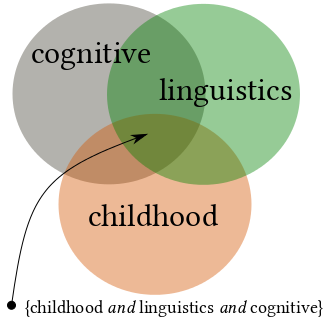
\includegraphics[width=.45\textwidth]{and3colors.png}
\end{center}

In the search depicted above, a student has requested articles that contain the 
subjects \textbf{cognitive}, \textbf{linguistics}, and \textbf{childhood}. 
Significantly, this particular search will only retrieve articles that contain 
\emph{all three terms}. This small subset of the larger subject sets is 
referenced by the arrow. All the information represented by the other portions 
of the three circles will be excluded. Thus, even if an article contains two of 
the three search terms, it will be excluded from the results.

\subsection{OR}
Unlike the \textbf{AND} operator, \textbf{OR} seeks to \emph{broaden} a search, 
as in this example:

\begin{center}
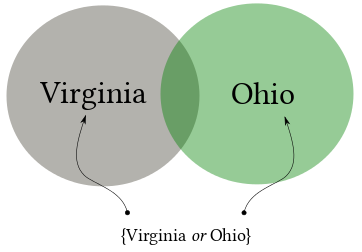
\includegraphics[width=.45\textwidth]{Orcolor.png}
\end{center}

In the search depicted above, a student has searched for the subjects Virginia 
\textbf{OR} Ohio. This search will return \emph{every} article having the 
subject of Virginia as well as \emph{every} article with the subject of Ohio. 
Unlike the \textbf{AND} search, where only articles containing \emph{both} 
terms are returned in the search results, the \textbf{OR} search yields every 
article on both subjects regardless of whether those subjects appear together 
in the same article. As a consequence, the \textbf{OR} search will produce far 
more results. 

Since the \textbf{OR} operator lacks precision, it is most often used in 
parenthetical searches, described below.

\subsection{NOT}
The Boolean operator \textbf{NOT} is used to \emph{subtract} or \emph{screen 
out} topics or keywords that are unwanted within the search results. 


\begin{center}
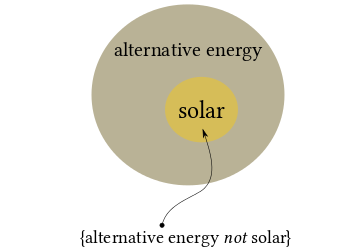
\includegraphics[width=.45\textwidth]{notcolor.png}
\end{center}


In the search depicted above, a student is researching alternative energy and 
wants to exclude any information dealing with solar energy. To remove all 
references to solar energy, the student has searched for \textbf{alternative 
energy}, but has removed any articles from the search results that contain the 
subject \textbf{solar} using the operator \textbf{NOT}. 

The \textbf{NOT} operator is helpful when you find your search results are 
"polluted" with unwanted items. This is often a problem when two distinct 
things share the same name. For example, if you were researching the Norse 
explorers known as the Vikings, you might discover that your search results 
include unwanted information about the Minnesota Vikings football team. You can 
subtract these unwanted results by searching for \textbf{Vikings not Minnesota} 
or \textbf{Vikings not football}.  

\subsection{Parenthetical Searches}

You can also use the various Boolean search terms in tandem using parenthetical 
constructions:

\begin{itemize}
\item (Ohio or Virginia) and unemployment
\item (cognitive and linguistics) not childhood
\end{itemize}
Such parenthetical searches follow the order of operations, like in math 
equations. In the first example, the search will first combine all the articles 
that are on the subjects of \textbf{Ohio} or \textbf{Virginia}, creating a 
large collection of search results. Afterward, the search term 
\textbf{unemployment} will be applied to that collection, yielding the final 
search results. Similarly, the second example creates a large collection of 
results that share the subjects \textbf{cognitive} and \textbf{linguistics}, 
then all the items having the subject \textbf{childhood} are removed from the 
results.

\subsection{Exact Phrase}

Most Internet search engines and library catalogs default to the \textbf{AND} 
operator when multiple terms are entered, even if it has not been typed by the 
user. For example, if you search for \textbf{artificial intelligence}, the 
search algorithm will actually use the search phrase \textbf{artificial 
\emph{and} intelligence} to produce your results. In some circumstances this 
may produce undesirable or imprecise results.

To avoid this problem, you can instruct your search engine to perform what is 
known as an \textbf{exact phrase search}. This is performed by placing 
quotation marks around the exact words that you are searching for. By searching 
for "artificial intelligence" your search results will only contain items that 
have that exact phrase within the document.

\subsection{Truncation and Wild Cards}
\begin{itemize}
\item manufact\** [truncation]
\item wom\**n [wild card]
\end{itemize}
If you search for the terms \textbf{steel and manufacturing}, your search 
results will not include results with the terms \textbf{manufacturer}, 
\textbf{manufacture}, \textbf{manufactured}, or \textbf{manufactures}. As a 
result, you may not discover articles or books that are important to your 
research. By truncating the word with an asterisk, you will gather all the 
relevant search results. 

Similarly, if you only search for wom\underline{en}, you will miss out on the 
all the texts that mention wom\underline{an}. However, using the wild card 
asterisk you will search both terms simultaneously.

\section{Finding a Book in the Library}

\subsection{The Library of Congress System}
Most research libraries use the Library of Congress (LC) classification system 
to organize their holdings. The Library of Congress assigns each book a unique 
\textbf{call number} consisting of a series of numbers and letters that help 
you locate them on the library's shelves. A typical call number will resemble 
the following: 

\begin{quote}
\hspace{.4in}{\huge F 24 .T39 1990}
\end{quote}

Let's break down the call number into its component parts:

\begin{quote}
\hspace{.4in}\begin{tabular}{ |l|l| }
  \hline
  F & Letter, or subject, line \\ \hline
  24 & Whole number line \\
  \hline
  .T39 & Cutter line \\ \hline
  1990 & Edition, or Date, line\\ \hline
\end{tabular}
\end{quote}

\begin{itemize}
\item \textbf{The Letter line} describes the subject matter, or discipline, of 
the book. It also indicates the section of the library where the book is 
shelved (consult your library's map and floorplan). The letter line will be 
between one and three letters long.
\item \textbf{The Whole number line} tells you which \emph{row} the book is on 
in the stacks. 
\item \textbf{The Cutter line} identifies the \emph{individual book}. The first 
letter of the Cutter line is usually the first letter of the author's last name.
\item \textbf{The Edition, or Date, line} tells you the book's year of 
publication. This line is used to distinguish between editions.
\end{itemize}

\subsection{How to Find a Book}
To find a book in the library, read the call number from left to right, using 
alphabetical and numerical orders. First, using the \textbf{Letter line}, 
determine the floor of the library where the book is shelved. Use the library's 
\href{http://www.bu.edu/library/mugar-memorial/about/floorplans/#f=floor-1}{\{fl
oorplan maps\}} to locate the proper section. Using our example call number 
above, we can determine that the \textbf{F} section is on the 4th floor of 
Mugar library. 

Once on the appropriate floor, use the \textbf{Whole number line} to find the 
row where the book is shelved in the stacks. Using the example call number, we 
will look through the stacks for the number 24. The floormaps are often helpful 
in locating the book's general location on the library floor. As you walk 
through the stacks, look on the ends of each row of books for signs describing 
the range of books held within the rows. You might, for example, see a sign 
reading:

\begin{center}
\hspace{.4in}{\huge F 7.4\textendash F 45.2}
\end{center}

Since \textbf{F 24} is within this range, our example book is in that row. Once 
in the proper row of shelves, proceed numerically until you find the 24s. 

Finally, using the \textbf{Cutter line}, proceed alphabetically until you find 
the Ts. Then proceed numerically until you find .T39, the address of our book. 

As you can see, the call number should be read from left to right using 
alphabetical and numerical orders. Thus, a book with a Subject line \textbf{F 
}would be shelved \emph{before} a book with a Subject line \textbf{FA.} 
Similarly, a Cutter line that reads \textbf{.T39} is shelved \emph{after} 
\textbf{.T21}. 

\begin{itemize}
\item \textbf{Remember, in decimals .7 is bigger than .21!}
\end{itemize}

Maps of the library's floorplans are affixed to the walls on each floor. Free 
paper maps of the library are available at the circulation desk of the library. 
You may also consult the 
\href{http://www.bu.edu/library/mugar-memorial/about/floorplans/#f=floor-1}{\{ma
ps and floorplans\}} online or with your computer or smartphone. 

\section{What if we don't have it?}
    
A common problem in academic research is discovering that a source that you 
require for a project is checked out, missing, or not owned by the library. 
There are a number of free services available to you when you encounter this 
problem.

\subsection{Boston Consortium Libraries}

A number of Boston-area colleges and universities have formed a library 
consortium designed to share resources and expand research options for the 
entire academic community. As students of Boston University, you may obtain 
borrowing privileges at any of the other participating libraries. 

To see if a book is available at another 
\href{http://www.blc.org/members/current-members}{\{BLC\}} library, use a 
service called \href{http://www.bu.worldcat.org}{\{WorldCat Local\}}. With this 
service you can search every library in the BLC simultaneously to see if the 
book you require is available at another local institution. If the book is 
owned by another school and is not checked out at the time, you may request 
that the item be sent to our library. To request a book, browse to the book's 
record in the WorldCat catalog and click the green button labeled "Request 
Item." Once Mugar's circulation desk receives the item, they will inform you 
through email that the text is ready for pickup.

\subsection{Boston Library Consortium Card}
If you would like to check out a book at one of the other BLC member libraries 
in person, you may obtain borrowing privileges by applying for a 
\href{http://www.bu.edu/library/services/ill/blc-cards}{\{Boston Library 
Consortium Card\}}. To apply, fill out the online form and you will be 
contacted when your card is ready for pickup at Mugar's circulation desk.

\subsection{Interlibrary Loan}
If there is a book or article you would like to read that is not available at 
any BLC library, you may request it from BU's Interlibrary Loan office. To 
request an item, visit the 
\href{http://illiad.bu.edu/illiad/bos/illiad.dll}{\{Interlibrary Loan\}} 
webpage, select the appropriate form (article, book, book chapter, etc.), and 
send your request electronically to the ILL office. The staff in the office 
will request your item from another library, who will ship the book to our 
library through the mail. 

\textbf{Please note}: Interlibrary Loan is the \emph{slowest} of all the 
available options for requesting research materials. Requests may take up to 
two weeks to be fulfilled. 


\section{Research Guides}

If you are performing research on a topic and do not know where to begin, 
Boston University Librarians have created an impressive collection of 
\href{http://www.bu.edu/library/guides/index-a-h.html}{\{Research Guides\}} 
that can help you find background information, periodical databases, and 
academic journals appropriate for your topic or discipline:

\begin{itemize}
\item\href{http://www.bu.edu/library/research/guides/research-guides/area-and-cu
ltural-studies/}{\{Area and Cultural Studies\}}
    
\item\href{http://www.bu.edu/library/research/guides/research-guides/arts-and-hu
manities/}{\{Arts and Humanities\}}

\item\href{http://www.bu.edu/library/research/guides/research-guides/management-
business/}{\{Business and Management\}}

\item\href{http://www.bu.edu/library/research/guides/research-guides/science-and
-engineering/}{\{Science and Engineering\}}

\item\href{http://www.bu.edu/library/research/guides/research-guides/social-scie
nce/}{\{Social Sciences\}}
\end{itemize}

\section{Peer Review}

Peer review is a form of quality control in academic publishing. Before books 
or articles are published, they experience a rigorous process of evaluation by 
a number of experts who have advanced training in the field of study in 
question. This scholarly review helps eliminate factual errors and other 
problems before the works are published. Thus, peer-reviewed works much more 
trustworthy than other sources of information. 

\subsection{How do you determine if a source is peer-reviewed?}

For novice researchers, distinguishing between peer-reviewed and other kinds of 
sources can be challenging. 

There are a number of things you can do to ensure that you are using 
peer-reviewed information. Many periodical databases, such as 
\href{http://www.jstor.org.ezproxy.bu.edu/jstor/}{\{JSTOR\}}, only contain 
peer-reviewed academic articles. Many other databases, such as 
\href{http://infotrac.galegroup.com.ezproxy.bu.edu/itweb/mlin_b_bumml?db=AONE}{\{Academic OneFile\}}, have a search limiters that can be selected to ensure 
that the search results only contain peer-reviewed sources. However, other 
databases lack clear indications about the nature of their sources. If you are 
confused about a source or database, ask your professor or one of the research 
librarians for assistance.

If those are not practicable, use these test criteria:
\begin{itemize}
\item Scholarly, peer-reviewed articles almost always publish the university 
affiliation of the professor/author/scientist. 

\item Scholarly articles \emph{always} have a bibliography page. 

\item Scholarly articles always contain citations and commonly have footnotes 
or endnotes. 

\item Generally speaking, if you can find the publication at the dentist's 
office or on an airport magazine rack, then it isn't scholarly or 
peer-reviewed. \emph{Time}, \emph{Newsweek}\textemdash even the \emph{New York 
Times}\textemdash are not considered peer-reviewed sources.
\end{itemize}

\section{The Oxford English Dictionary}

The \href{http://www.oed.com.ezproxy.bu.edu}{\{OED\}} is, without question, the 
greatest and most complete dictionary ever created. Many generations of 
scholars have made it their life's work. The OED systematically traces the 
etymology of words in the English language. 
\href{http://en.wikipedia.org/wiki/Etymology}{\{Etymology\}} is "the study of 
the history of words, their origins, and how their form and meaning have 
changed over time." Thus, with the OED you can see when a word entered or 
exited the English language and how its meaning evolved over time. 

The OED is quite helpful when you are reading a novel, poem, or document that 
was written in a time period distant from our own. Since words fall out of use 
and the meanings of words change over time, it can often be difficult to 
interpret the meaning of the texts we read from the past. The OED exists to 
help us with this problem: you can think of it as a dictionary with a built-in 
time machine. 


\section{Helpful Research Suggestions}

\subsection{Not all sources are equal}

How do you know if you can trust your source? Here are some suggestions for 
critically examining your sources:

\begin{itemize}
\item \textbf{Examine the credentials of the author}. What is their educational 
background? Do they have an advanced degree in the subject that they are 
writing about? Are they affiliated with any major institutions\textemdash such 
as a university or government department? Does the author have a respected 
publication record that is frequently cited by other experts in the field?

\item \textbf{Examine the date of publication}. When was the book or article 
you are reading published? Since new discoveries and ideas are produced every 
day, it is important to consult the most recent sources on your research 
subject. Generally, the most current source should be preferred over older 
sources.

\item \textbf{Determine if the source has been peer-reviewed}. Peer review is a 
form of quality control in academic publishing. It ensures that the information 
that is published has been properly evaluated and vetted by a number of other 
professionals in the field. A peer-reviewed source should be preferred over any 
other kind of information.

\item \textbf{Be wary of Internet sources}. If your source comes from the 
Internet, you should take care to verify its trustworthiness. Most sites on the 
Internet are not peer-reviewed sources of information. Misleading, politically 
motivated, and even propagandistic content often masquerades as objective 
information on blogs, websites, and discussion boards. 
\end{itemize}

\subsection{Taking notes}

Now that you have some research materials in front of you, either at the 
library or at home, it's time to make them useful to you. Before placing source 
materials in your essay, take good notes instead by using summary, paraphrase, 
and judicious quotation to take ownership of the source materials. Ensure that 
you cite appropriately and that your summaries and paraphrases use your own 
original language. This intermediary step before writing the essay saves you 
time and helps you avoid plagiarism.

If you'd keep organized notes on your computer, try the free, open-source 
program called \href{http://rasm.ods.org/keepnote}{\{Keepnote\}}.

\subsection{Raid the Bibliography}

Occasionally, students find one or two sources on a topic and then despair of 
finding any more. However, with just one excellent article or book, you can 
easily generate additional research leads. When you find a book or article that 
relates to your project, scour the bibliography to see what books and articles 
the author used to produce his or her work. Make lists of the most promising 
sources by writing down all the bibliographic information in a research 
journal. Locate these sources in the library and then repeat the process. By 
using this technique of routinely following up on sources cited in 
bibliographies, you can generate a surprisingly large number of books and 
articles on your topic in a relatively short time.

\subsection{Keep a Research Journal}

Keeping a research journal is an important habit to develop. Every student or 
professor has had the unsettling realization that they have used a quotation in 
their writing but have no recollection of where the quote came from. Many hours 
can be consumed retracing steps. Frequently, source materials are never located 
again. To avoid this problem, keep a research journal where you record the 
bibliographic information of each source you read or browse. This way you can 
quickly locate the information again. 

Although a paper notebook works well as a research journal, there are some very 
promising electronic alternatives. This bibliographic software can maintain a 
record of your sources, help you take notes, and even produce perfectly 
formatted bibliography pages for your essays. 

For Mac users, there is \href{http://www.sonnysoftware.com/}{\{Bookends\}}. PC 
users should consider \href{http://www.biblioscape.com}{\{Biblioscape\}}. 
However, the free and open-source option known as 
\href{http://zotero.org}{\{Zotero\}} is perhaps the best option of all.



%-----------------------------------
%ANNOTATING READINGS
%-----------------------------------


\chapter{Annotating Texts}

\begin{quote}
\small
"We believe the best way to work on a difficult text is by rereading \dots but you can also work on the difficult text by writing, by taking possession of the work through sentences and paragraphs of your own, through summary, paraphrase, and quotation, by making another writer’s work part of your work." (12)

--Bartholomae and Petrosky, "Introduction." \emph{Ways of Reading: An Anthology for Writers
Critical Reading}

\end{quote}

Analysis requires breaking an argument into smaller parts so that you can understand how those parts work together to make the whole (or fail to do so). The best way to begin this process is to write while you read in the form of underlining and the use of marginal notes and a system of symbols (made on the pages of the document itself). There is no right or wrong way to mark up a text, but you should develop a system that you are comfortable with and try to stick with it. Writing while you read will help you stay focused and read critically. In fact, I would argue that if you are not writing while you read — not “taking possession” of a text by putting it into your own words through annotation, summary, paraphrase, and quotation — then you are not really reading at all.

\subsection{Reading to reduce}

Your objective in annotation is to provide a plan for reducing a long, unwieldy document into something small and useful for study. I commonly underline the thesis once I find it. And, as I read, I place a large dot next to pieces of evidence or statements/assertions that are being used to support the thesis. I always place some kind of keyword or short statement next to the main argumentative moves that the essay makes. I further put a check mark or exclamation point next to statements that I find important or noteworthy. Sometimes I draw arrows to connect parts of the essay. In addition to marking up a text for later use, I ask questions in the margins or note places where I become confused. This is helpful later, on your second reading, since you can pay more careful attention to the passages that gave you trouble. I also write my thoughts as they occur to me and state objections to things which seem problematic. Sometimes I try to connect an idea in one text with the idea(s) in another (I may find places where I can compare/contrast the thinking of two writers). As you can see, the process of annotation keeps me engaged, active, and alert--key components in critical thinking. 

Of course, this is only the system that I developed. Feel free to use whatever symbols or markings that you prefer. However, it is absolutely critical that you develop some method of marking up a text to aid in the critical analysis of the challenging, dense, readings that you will encounter in college and throughout your life as a citizen of the world.

\subsection{Reduction: making a critical outline}

After I go through this process of marking up a text, I usually have a pretty solid understanding of the author's argument and my response to it. If this is an important essay or if I plan to use it in my own writing, I will put it through a process of reduction, where I try to trim the argument down to its bare essentials. With any luck, your annotations will guide your efforts to reduce the argument. On a separate piece of paper or a computer document I create a critical outline that aims to reduce the entire argument to its main idea and brief statements of paraphrase, summary, and significant quotations. I carefully note the page numbers where these summaries, paraphrases and quotations are taken from for future use in my own writing.

Of course, as you write this critical outline you will not only try to reduce the main points of the argument, you will also ask questions and make observations of the text. You should note the argumentative points that you find yourself strongly agreeing or disagreeing with and your reasons for doing so. You might see a logical inconsistency or want the author to provide more evidence for his or her claims. You might make a note to perform some research at the library or on the Internet on an unfamiliar concept or event mentioned in the argument. Ultimately, however, you will want to determine if the argument you have read is persuasive and provide the reasons why.

At the end of this process, you should have a simplified---but objective and accurate---version of the essay that has been ruthlessly cut down to its bare essentials as well as a number of critical observations, questions, and ideas that have emerged in your process of reading. By the time you reach this stage and read over your notes, you will have taken great strides toward mastering the argument. Of course, if the essay is difficult, you may have to repeat the process until you have a breakthrough. I cannot emphasize enough how helpful this process is. It will help you come to a greater understanding of the text’s claims and weaknesses while also activating your long-term memory.


%----------------------------------------------------------------------------------------
% Grading Rubric
%----------------------------------------------------------------------------------------

\chapter{Grading Rubric}


The following grading rubric has been adopted from 
\href{http://www2.winthrop.edu/english/WritingProgram/rubric.htm}{\{Winthrop University's Writing Program\}}:

\section{The A paper}
The A paper is superior work that far exceeds the requirements of the assignment. This 
paper tackles the topic in an innovative way, with an appropriate sense of audience 
and an effective plan of organization. The writer has clearly used the elements of 
reasoning to generate material for developing as well as structuring the paper. When 
evaluated, the paper meets the highest standards of critical thinking. For example, the 
point of view and purpose are clear. It outlines the question at issue and assumptions 
with precision. Its information is accurate, and its concepts are relevant. It reaches 
sufficient conclusions and interpretations. Its implications and consequences are deep 
and broad. All elements can be judged against the standards very favorably. When the 
writer uses source materials in the A paper, he/she demonstrates complete 
understanding of potential critical thinking impediments and also illustrates an insightful 
understanding of the elements of reasoning present in the source. The writer reveals 
an understanding of the stated and unstated concepts and/or assumptions that are an 
essential aspect of alternative perspectives and shows a sophisticated analysis of the 
information and conclusions used to support the source’s main argument. The writing 
style is energetic and precise; how the writer says things is as excellent as what the 
writer says. There is evidence of careful editing, since the paper contains few 
grammatical and/or mechanical errors. Research materials, if used, are correctly 
documented \dots.

\section{The B paper}

The B paper is above-average work that more than meets the requirements of the 
assignment. It has a clear sense of topic, audience, and purpose, with sound 
organization, good evidence, and good analysis and/or argument. As in the A paper, this 
writer has clearly used elements of reasoning to generate material for developing the 
paper, although not to the extent of the superior A paper. Similarly, all elements can be 
judged against the standards favorably. When the writer uses source materials, he/she 
demonstrates complete understanding of potential critical thinking impediments, but 
illustrates a less sophisticated understanding of the elements of reasoning present in 
the source. The writer reveals an understanding of the source’s assumptions and 
conclusions, but falls somewhat short in recognizing the stated and unstated concepts 
and/or assumptions of the argument. The writing style is clear and precise, and the 
paper shows evidence of careful editing, since the essay contains few grammatical 
and/or mechanical errors (although an otherwise superior paper can have errors that 
lower the overall grade). Research materials, if used, are correctly documented \dots.
\section{The C paper}
The C paper is adequate, average work that meets the requirements of the assignment. 
The paper has a clear sense of topic, audience, and purpose, with a generally sound 
organization, although problems with focus may exist. The evidence is adequate, but 
not as specific as in an A or B paper, and the analysis and/or argument is not as fully 
developed. This paper deals with the elements of reasoning as outlined above, although 
not to the extent of the A and/or B paper, and some elements may not be fully 
addressed. While the paper minimally meets the standards of critical thinking, it may 
not address some of these standards fully. When the writer uses source materials, 
he/she demonstrates a basic understanding of potential critical thinking impediments, 
but reveals only a rudimentary understanding of the elements of reasoning present in 
the source. The writing style is clear, although there may be problems with sentence 
construction or word choice. Though the writer has edited the paper, remaining errors 
may affect the ability to communicate. Research materials, if used, are correctly 
documented \dots.

\section{The D paper}

The D paper is below average work that demonstrates an attempt to fulfill the 
assignment and shows some promise, but does not meet the requirements of the 
assignment. The paper may have one or more of the following weaknesses. There may 
be problems with the sense of topic, audience, or purpose. The paper may not 
adequately address the elements of reasoning and the standards of critical thinking as 
outlined above. It may have a general or implied thesis, but the idea may be too broad, 
vague, or obvious. The organizational plan may be inappropriate or inconsistently carried 
out. Evidence may be too general, missing, irrelevant to the thesis, or inappropriately 
repetitive. The analysis and/or argument may be underdeveloped. The style may be 
compromised by repetitive or flawed sentence patterns and/or inappropriate word 
choice and confusing syntax. Grammatical and mechanical errors may interfere with 
readability and indicate a less-than-adequate attempt at editing or an unfamiliarity with 
some aspects of Standard Written English. Research materials, if used, may not be 
completely or accurately documented \dots.

\section{The F paper}

The F paper is unacceptable work that does not meet the requirements of the 
assignment. It exhibits one or more of the following weaknesses. It may not meet the 
purpose of the assignment. It may be an attempt to meet the requirements of the 
assignment, but have no apparent thesis or a self-contradictory one, or its point may 
be general or obvious and suggest no serious engagement with the topic. The paper 
fails to address the elements of reasoning and the standards of critical thinking as 
outlined above. It may display little or no apparent sense of organization; it may lack 
development; evidence may be inadequate, inappropriate, or may consist of 
generalizations, faulty assumptions, or errors of fact. The style suggests serious 
difficulties with fluency, which may be revealed in short, simple sentences and 
ineffective word choice. Grammatical/mechanical errors may interfere with reader 
comprehension or indicate problems with basic literacy or a lack of understanding of 
Standard English Usage. Research materials, if used, may not be handled responsibly 
and/or documented appropriately \dots.

%----------------------------------------------------------------------------------------
% END OF SECTION
%----------------------------------------------------------------------------------------



\end{document}